We derive upper limits on the SM gluon-fusion Higgs boson production cross section 
times the $\hww\to 2\ell2\nu$ branching ratio in the $115 < m_H < 300 \GeVcc$ mass range. 
The results are presented in terms of the ratio of the limits to the rate predicted 
by the SM as a function of the Higgs boson mass corresponding to an integrated 
luminosity of 1 $\ifb$ as a bench mark. 

The limits are derived with a statistical method based on Bayesian
inference~\cite{bayesian}, using a likelihood function from the
expected number of observed events modeled as a Poisson random
variable whose mean value is the sum of the contributions from signal
and background processes. We account for systematic
uncertainties in a form of nuisance parameters with a log-normal
pdf. Results are reported with a flat signal {\it prior}. To perform
the computation of the limits, the software package LandS~\cite{lands}
is used.

We perform the analysis in two ways: (a) taking the signal and background predictions directly 
from the simulation, (b) taking the signal and background predictions from the data results 
(see Section~\ref{sec:dataresults}) and scale them to 1 $\ifb$.
In the first case, the expected upper limits at 95\% C.L. for the cut based analysis are
shown in Figure~\ref{fig:cutbase_uls}. The expected upper limits at
95\% C.L. for the multivariate based analysis are shown in
Figure~\ref{fig:mvabase_uls} for a case where we apply a cut on the
discriminating variable. The expected upper limits at 95\% C.L using 
the shape of the multivariate discriminant variable are shown in 
Figure~\ref{fig:mvashape_uls}. The median of the 
confidence level distribution is always used to evaluate the expected upper limits.

\begin{figure}[!htbp]
\begin{center}
   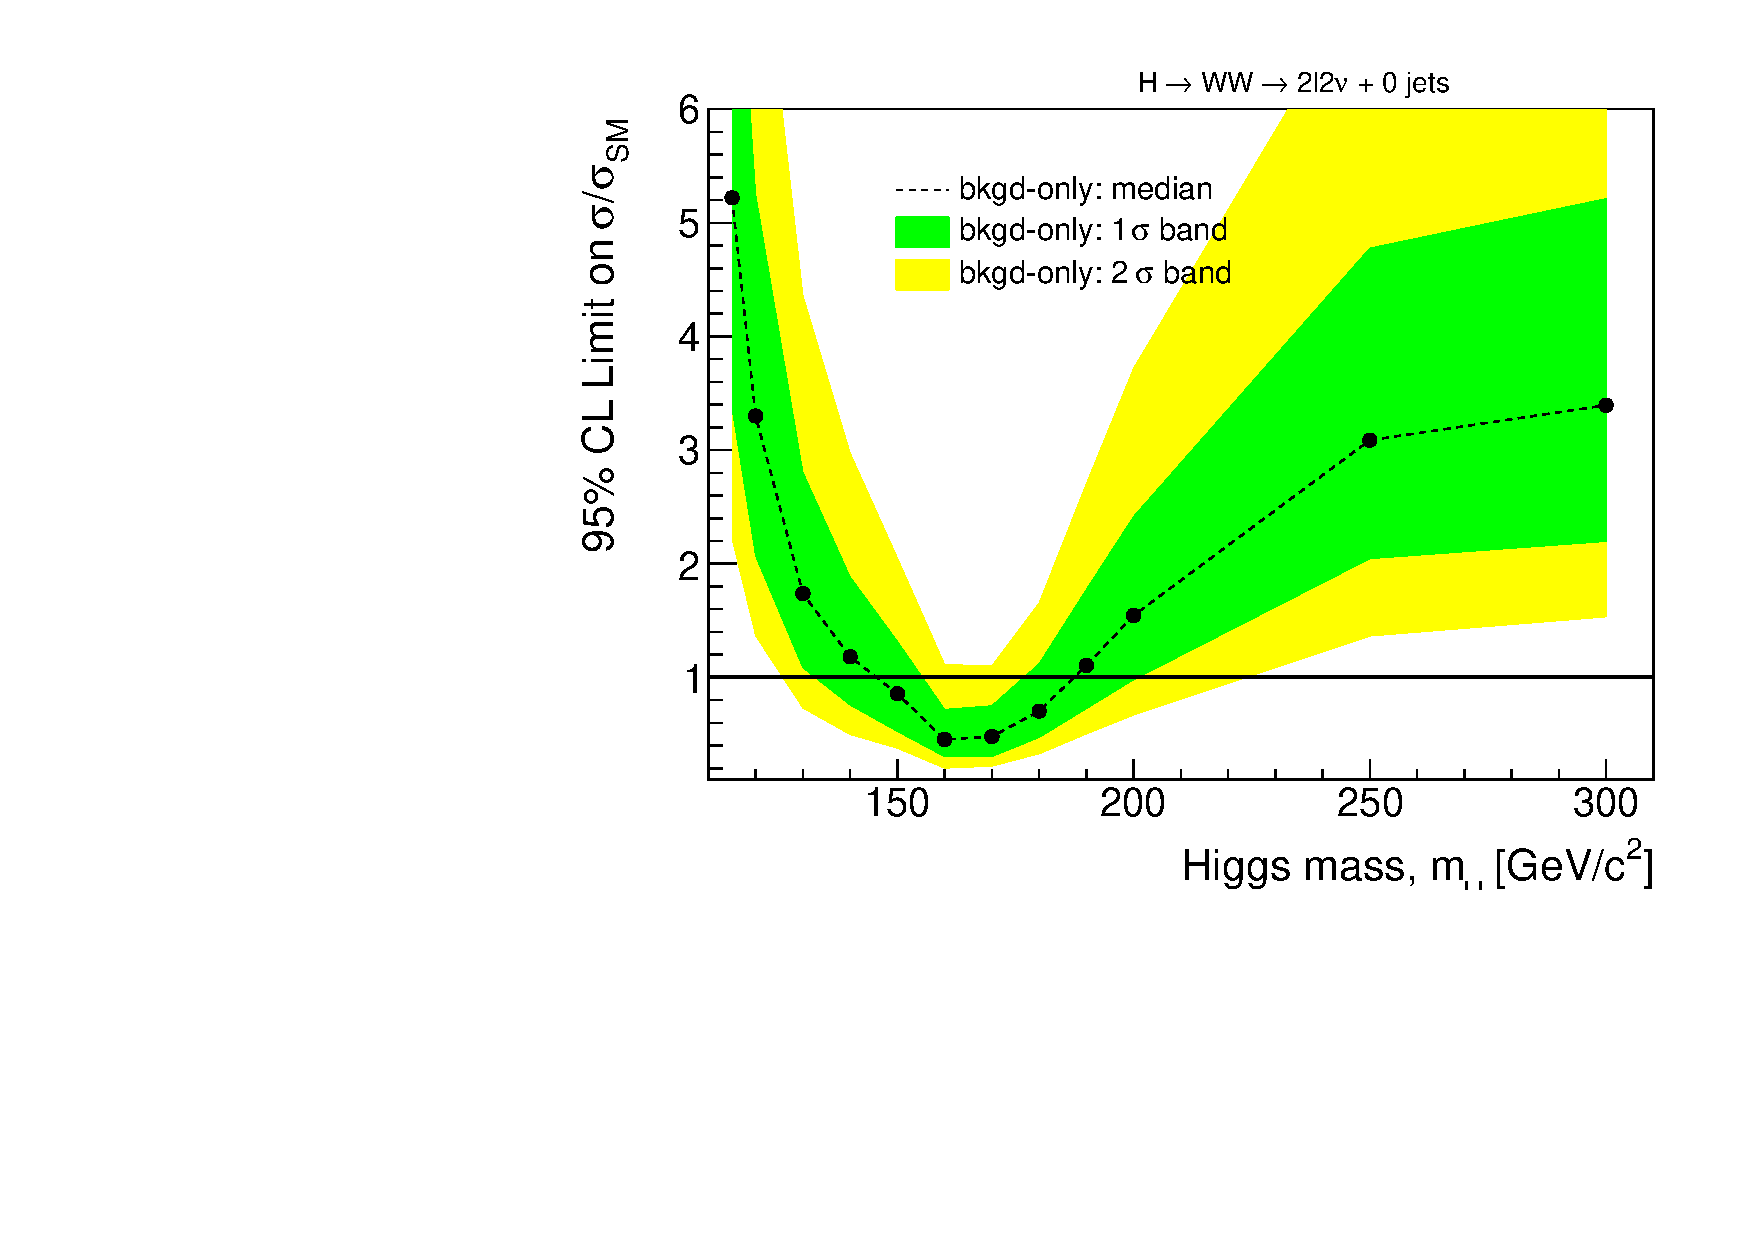
\includegraphics[width=0.49\textwidth]{figures/limits_0j_1000pb_cut_1.pdf}
   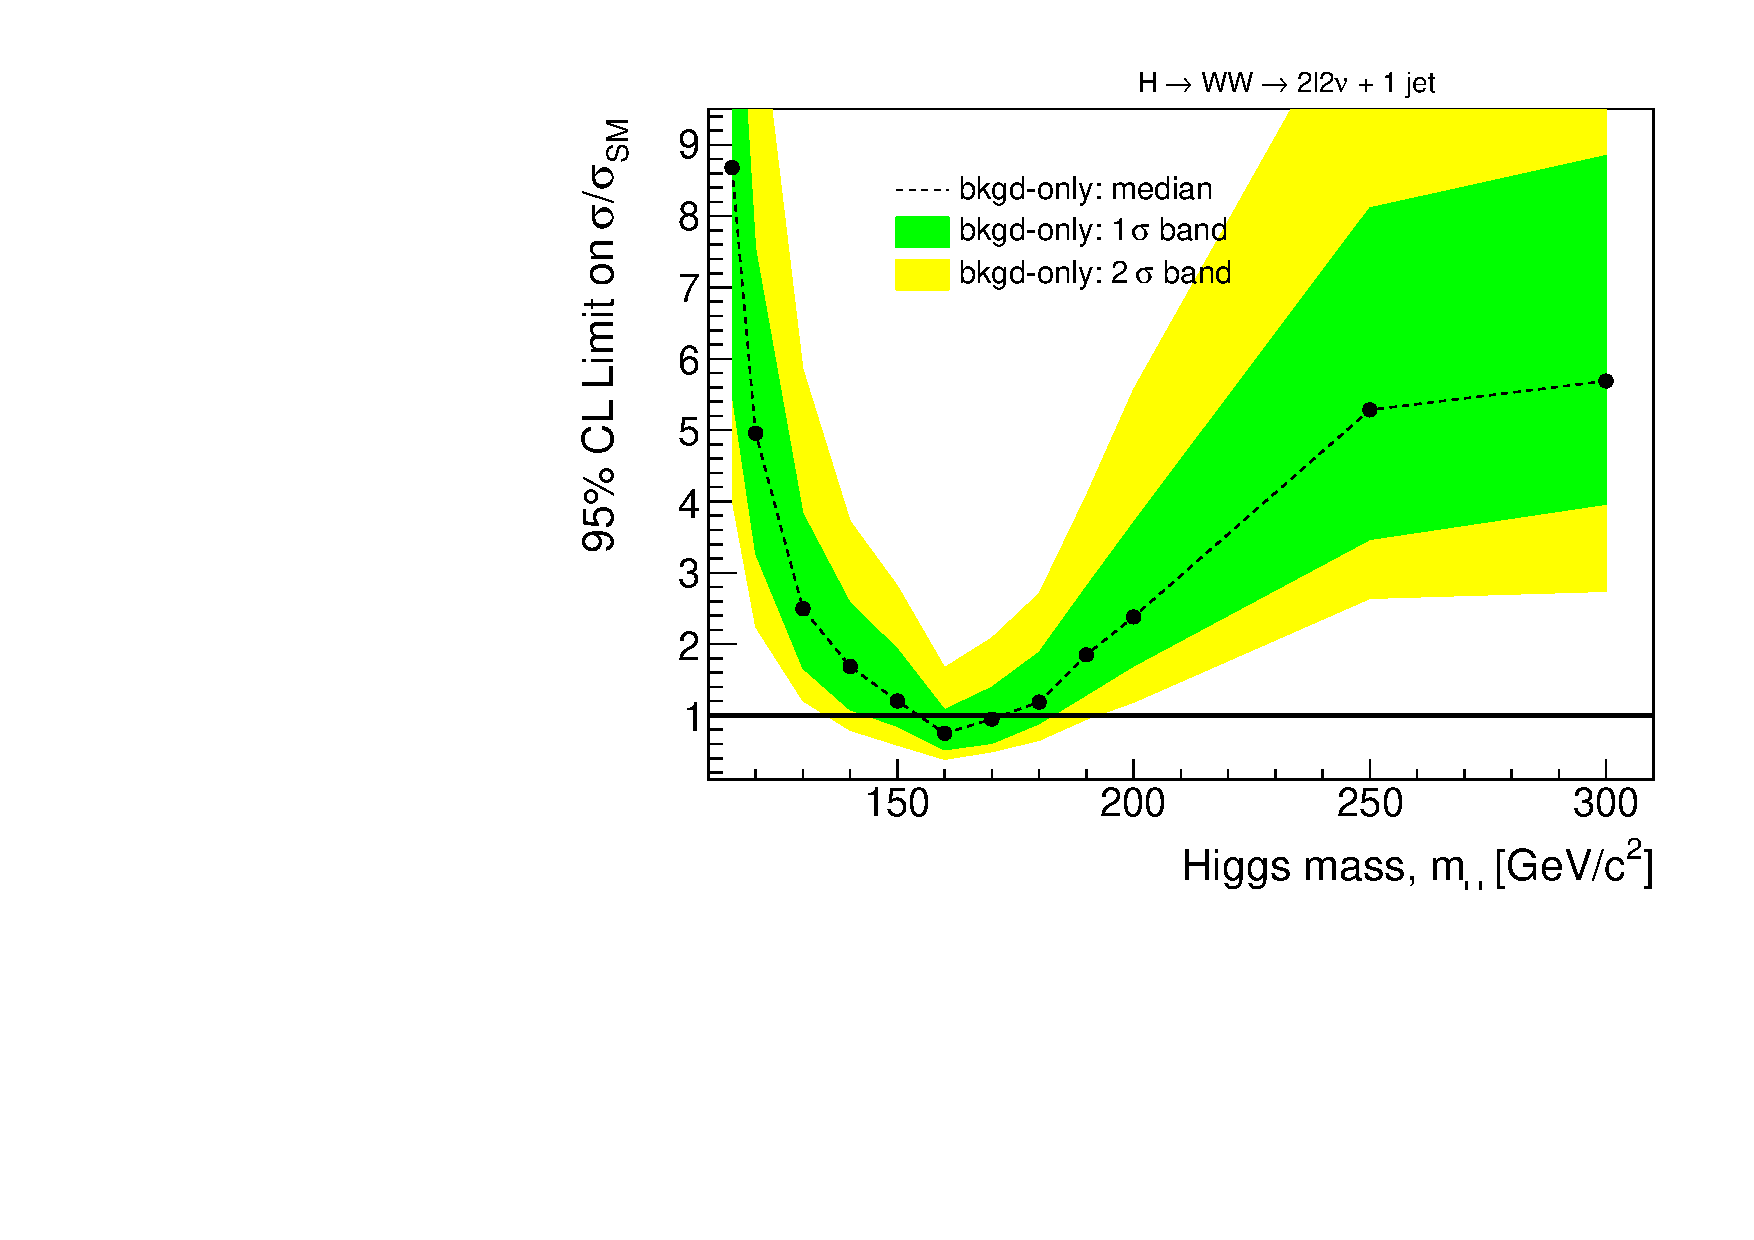
\includegraphics[width=0.49\textwidth]{figures/limits_1j_1000pb_cut_1.pdf}
   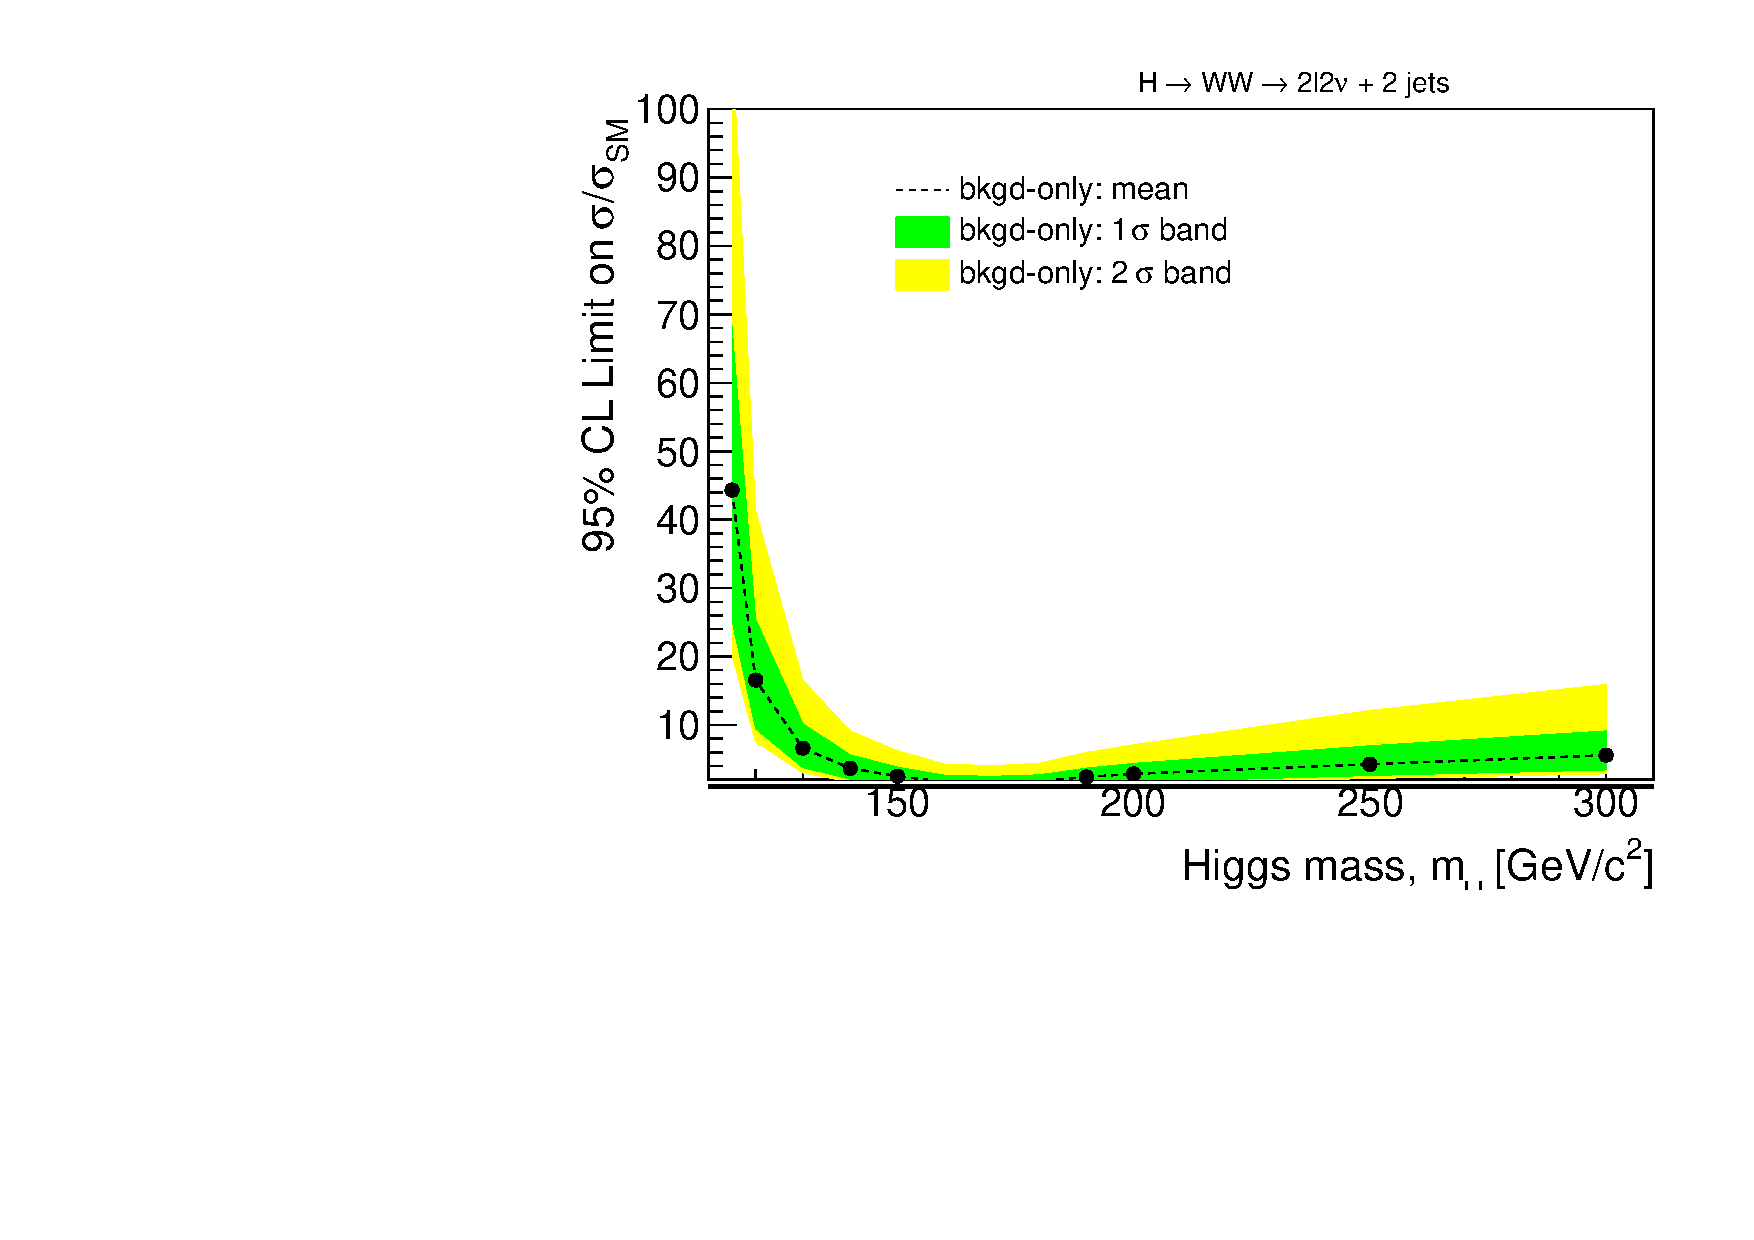
\includegraphics[width=0.49\textwidth]{figures/limits_2j_1000pb_cut_1.pdf}
   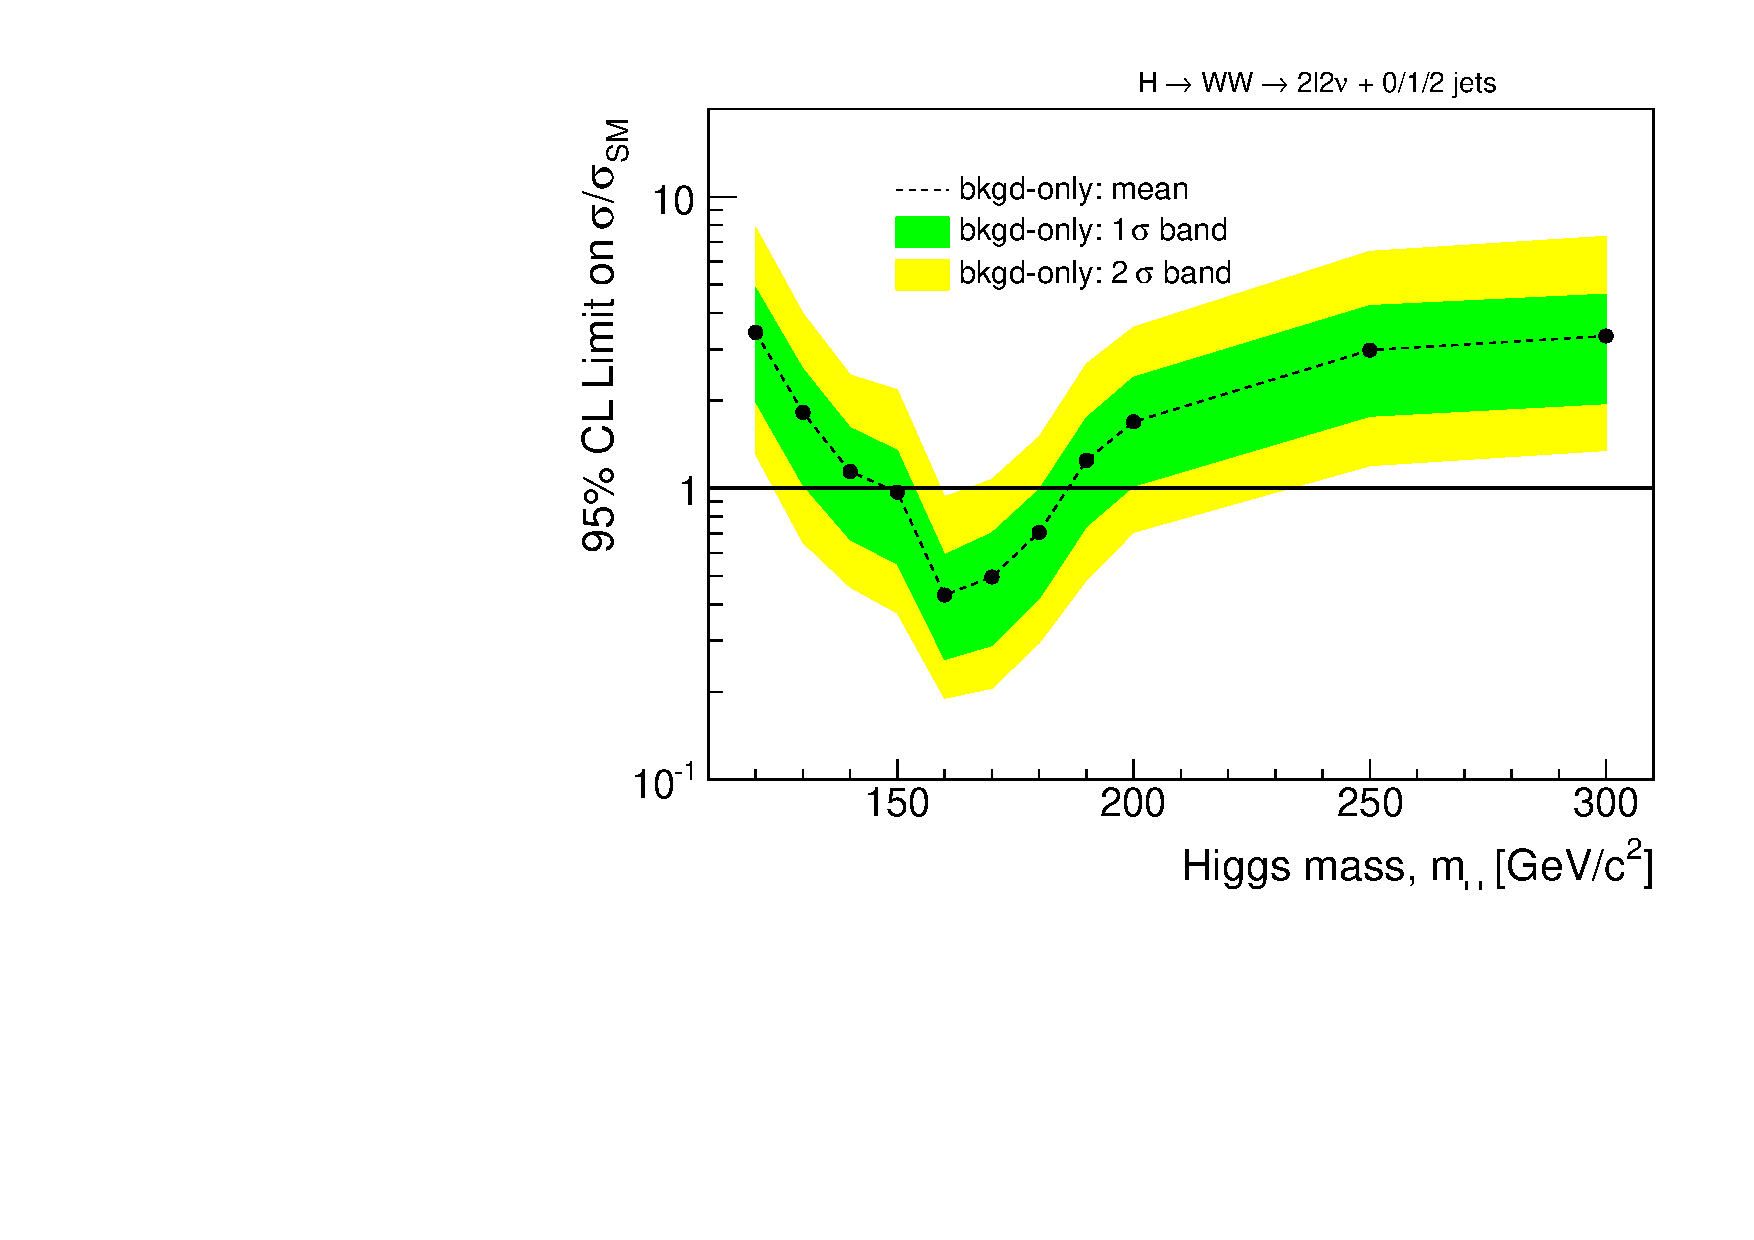
\includegraphics[width=0.49\textwidth]{figures/limits_nj_1000pb_cut_1.pdf}
   \caption{Cut based analysis expected upper limits at 95\% C.L. for 1\ifb\ of data. Top left plot 
   is the result for the 0-jet bin, top right plot is the result for the 1-jet bin, bottom left plot 
   is the result for the 2-jet bin and, bottom right plot is the combined result. The results 
   are based on the signal and background predictions directly from the simulation.}
   \label{fig:cutbase_uls}
\end{center}
\end{figure}

\begin{figure}[!htbp]
\begin{center}
   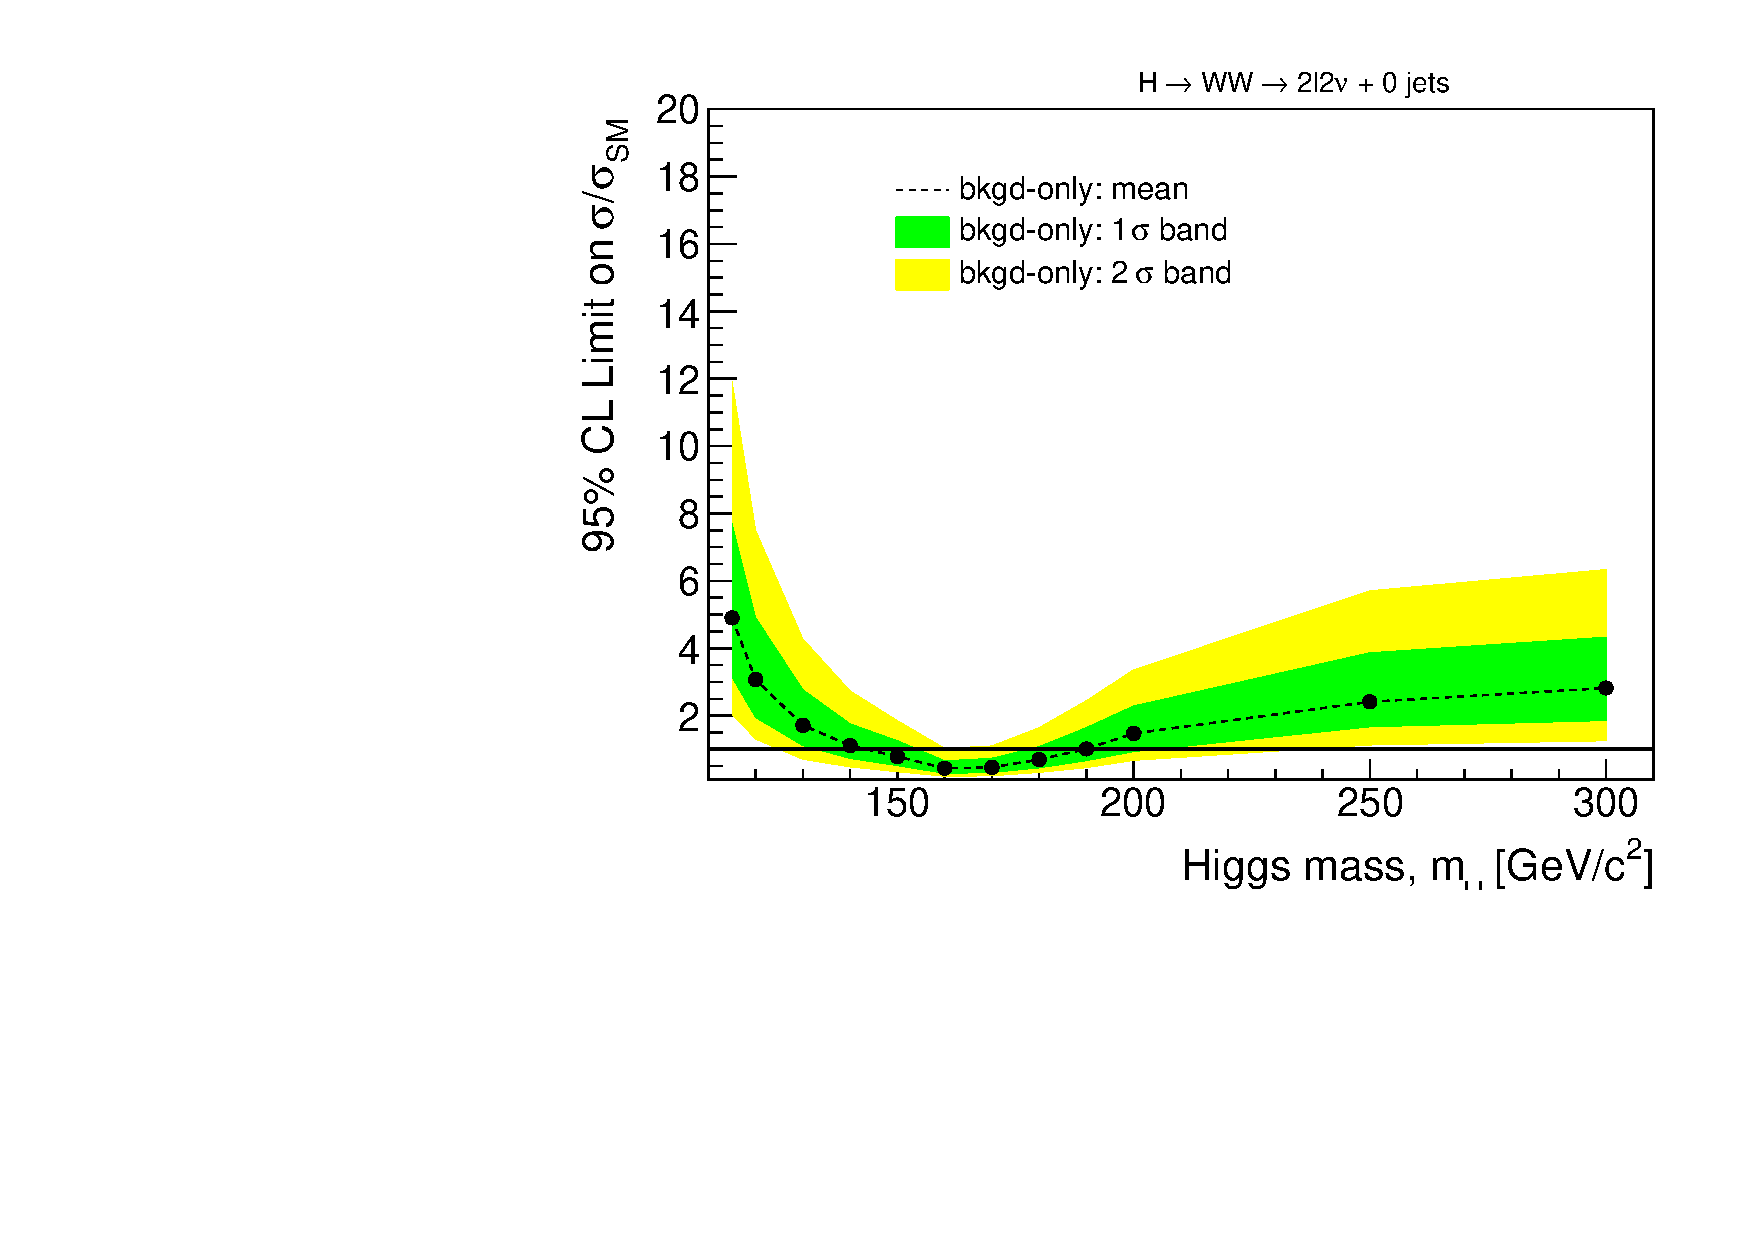
\includegraphics[width=0.49\textwidth]{figures/limits_0j_1000pb_mva_1.pdf}
   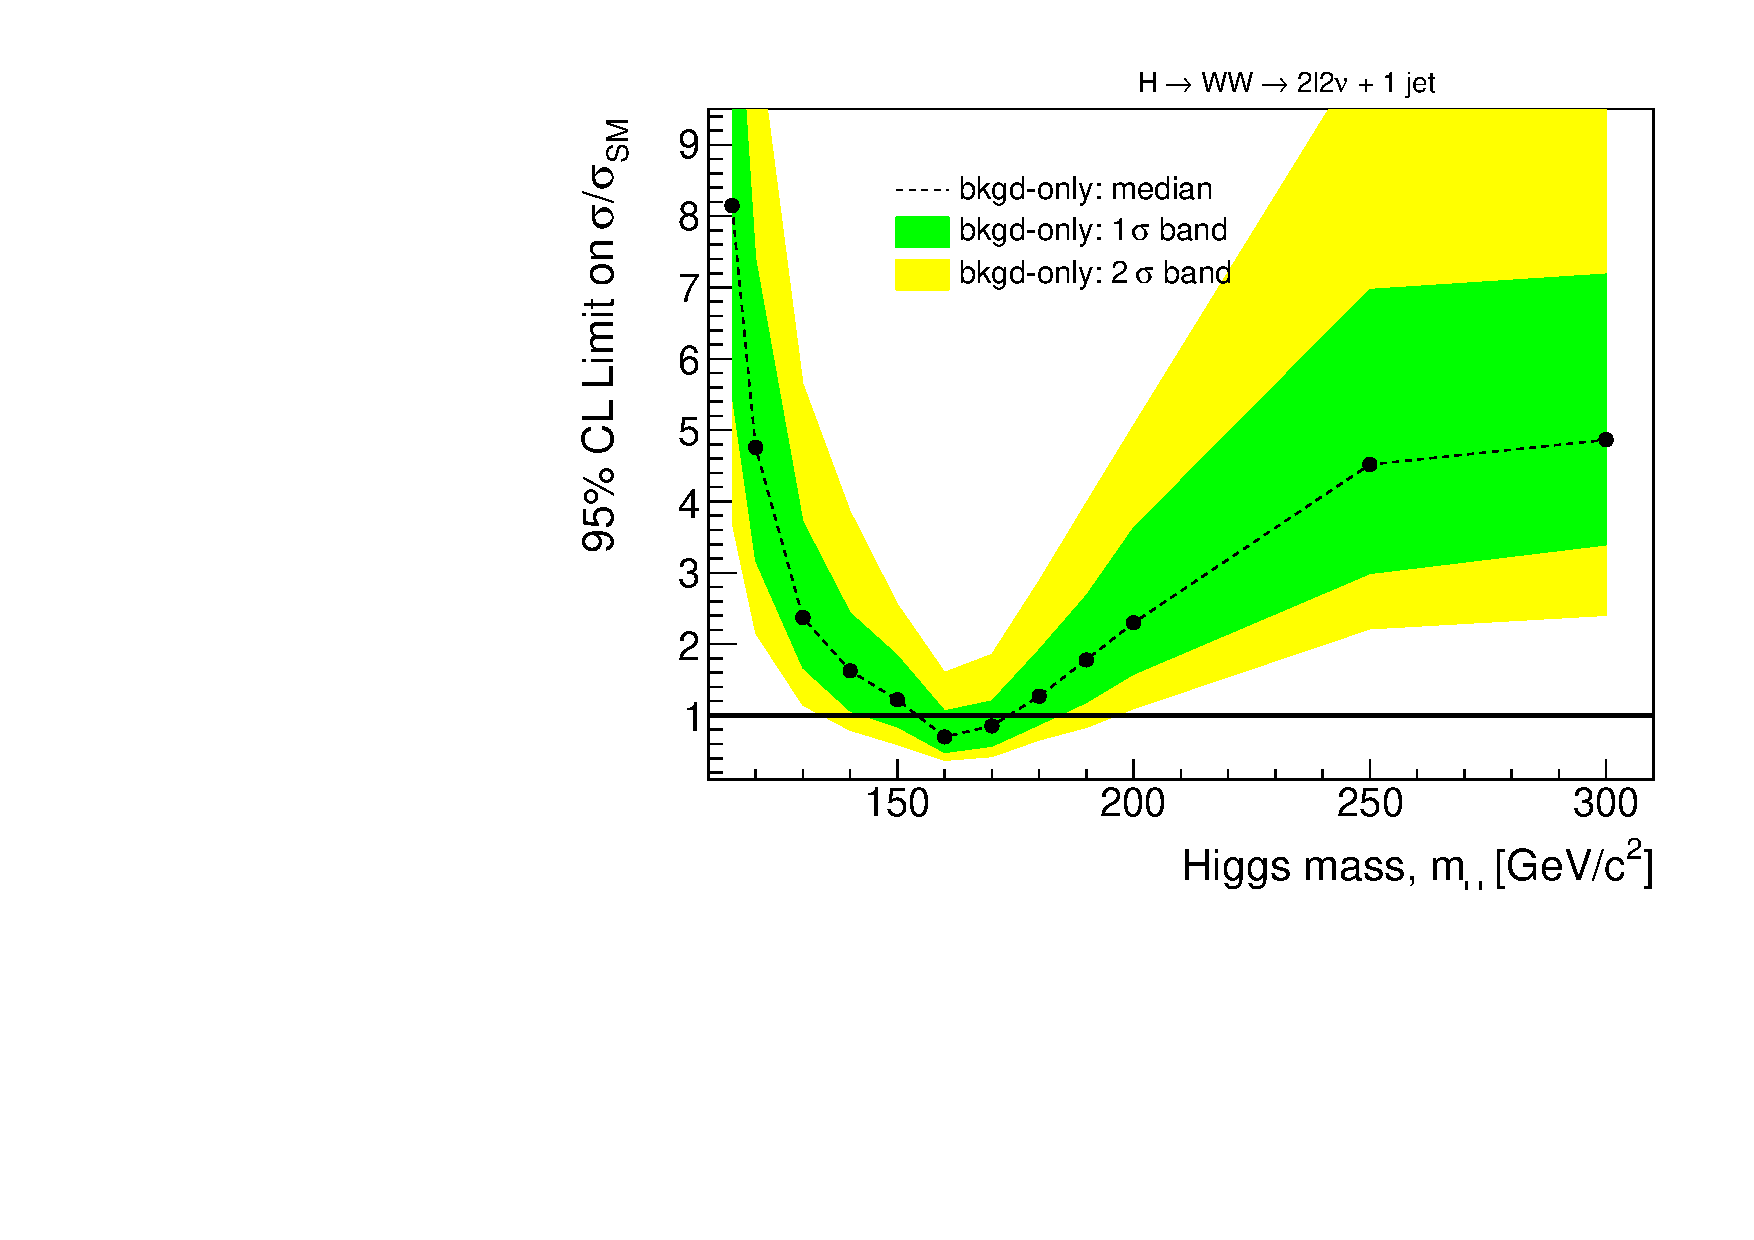
\includegraphics[width=0.49\textwidth]{figures/limits_1j_1000pb_mva_1.pdf}
   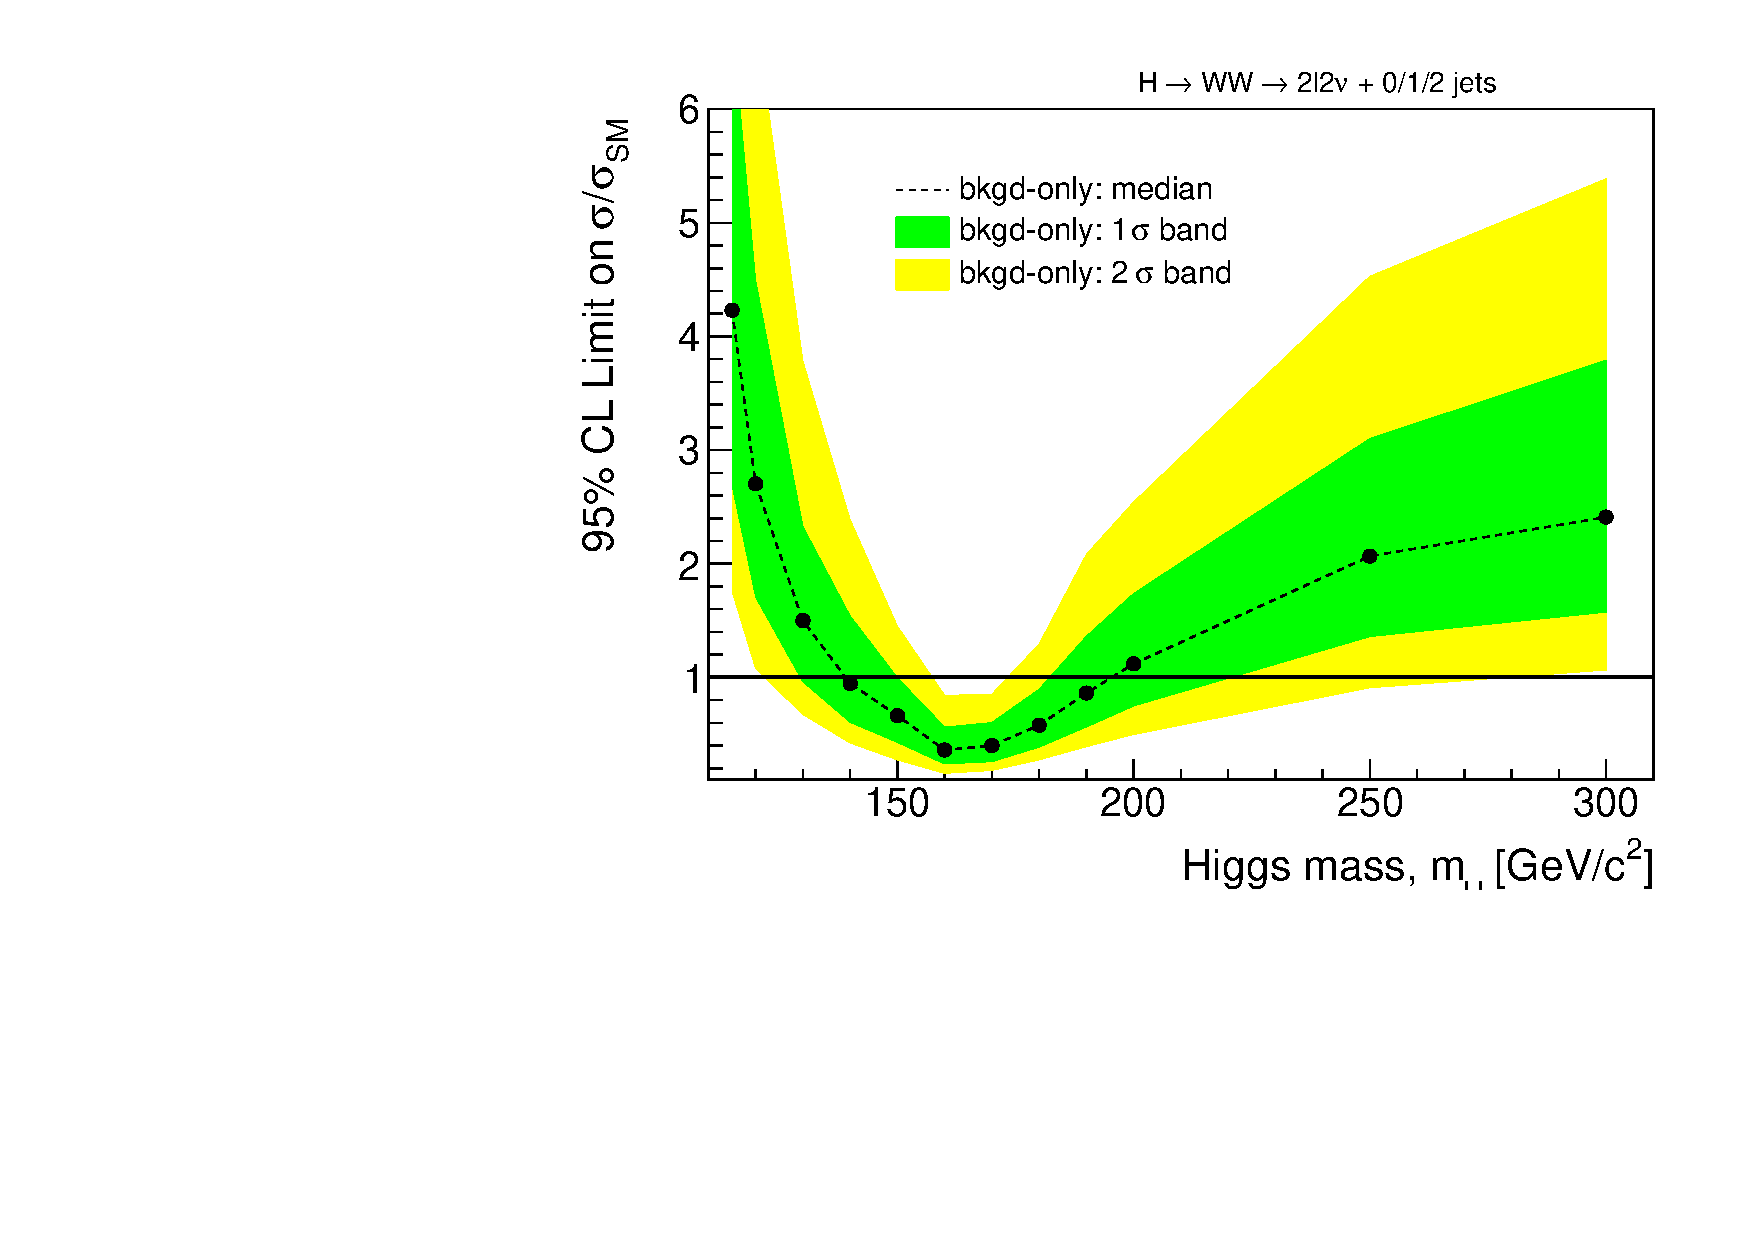
\includegraphics[width=0.49\textwidth]{figures/limits_nj_1000pb_mva_1.pdf}
   \caption{Multivariate cut-based analysis expected upper limits at 95\% C.L. for 1\ifb\ of data. Top left plot 
   is the result for the 0-jet bin, top right plot is the result for the 1-jet bin, and 
   bottom plot is the combined result including the cut based 2-jet bin analysis. The results 
   are based on the signal and background predictions directly from the simulation.}
   \label{fig:mvabase_uls}
\end{center}
\end{figure}

\begin{figure}[!htbp]
\begin{center}
   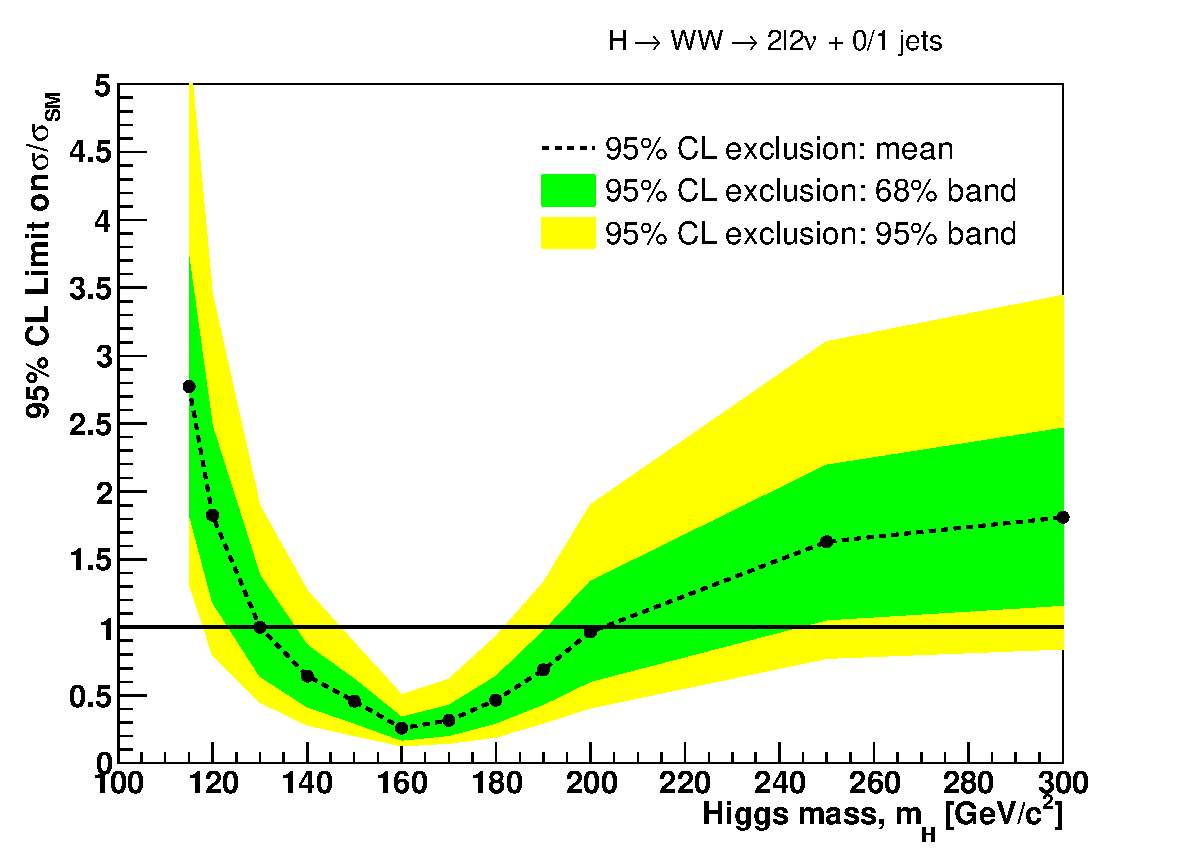
\includegraphics[width=0.49\textwidth]{figures/limits_0j_1000pb_shape.pdf}
   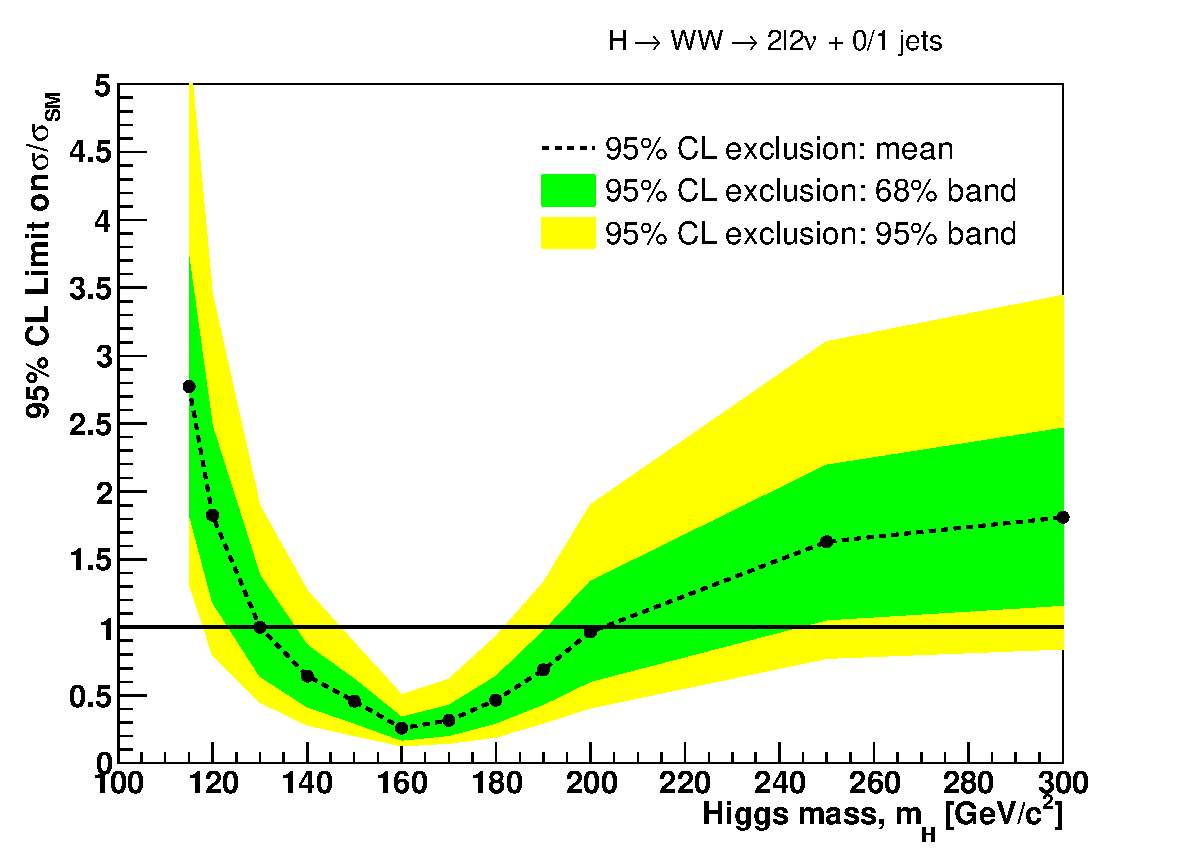
\includegraphics[width=0.49\textwidth]{figures/limits_1j_1000pb_shape.pdf}
   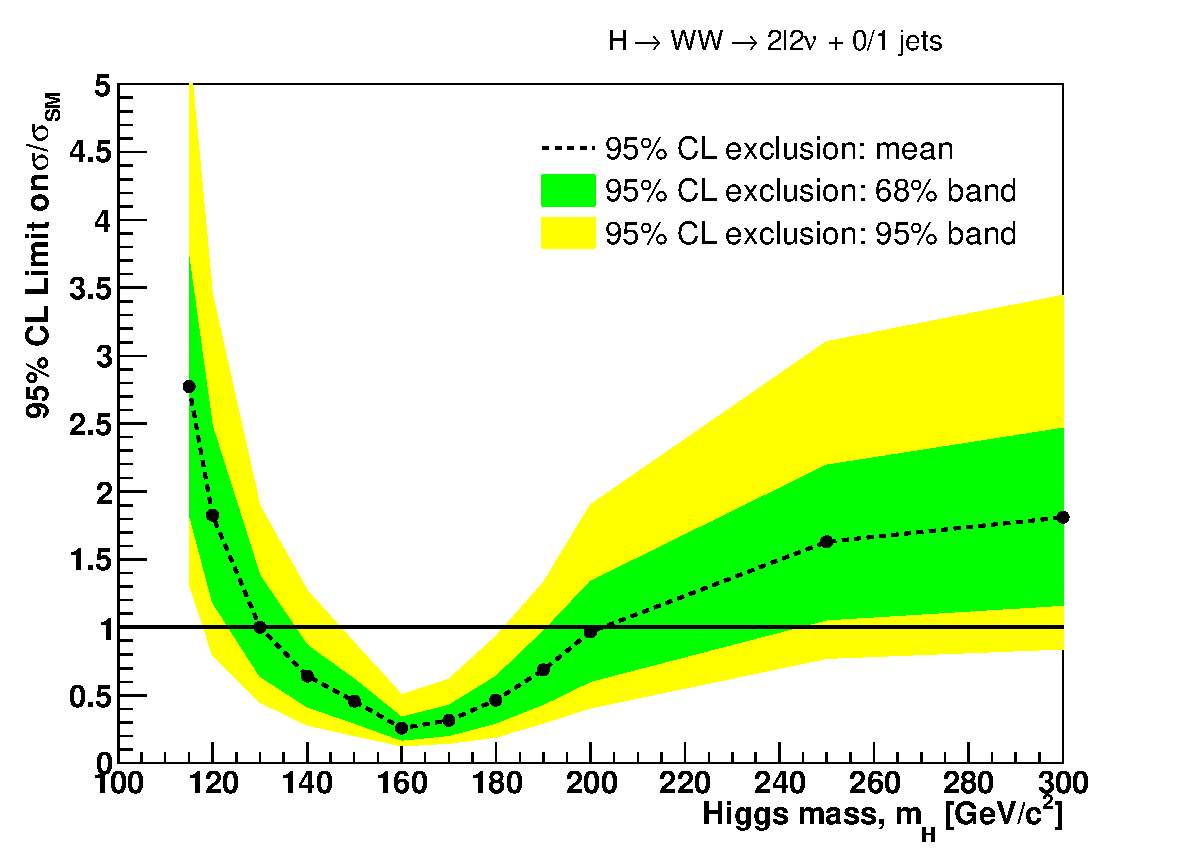
\includegraphics[width=0.49\textwidth]{figures/limits_nj_1000pb_shape.pdf}
   \caption{Multivariate shape analysis expected upper limits at 95\% C.L. for 1\ifb\ of data. Top left plot 
   is the result for the 0-jet bin, top right plot is the result for the 1-jet bin, and 
   bottom plot is the combined results. The results 
   are based on the signal and background predictions directly from the simulation.}
   \label{fig:mvashape_uls}
\end{center}
\end{figure}

The expected upper limits at 95\% C.L. for the cut based analysis using the data 
corrections for the signal and backgrounds are shown in 
Figure~\ref{fig:cutbase_uls_datalike}. The expected upper limits at
95\% C.L. for the multivariate based analysis are shown in 
Figure~\ref{fig:mvabase_uls_datalike} for a case where we apply a cut on the 
discriminating variable. The expected upper limits at 95\% C.L using 
the shape of the multivariate discriminant variable are shown in 
Figure~\ref{fig:mvashape_uls_datalike}.

\begin{figure}[!htbp]
\begin{center}
   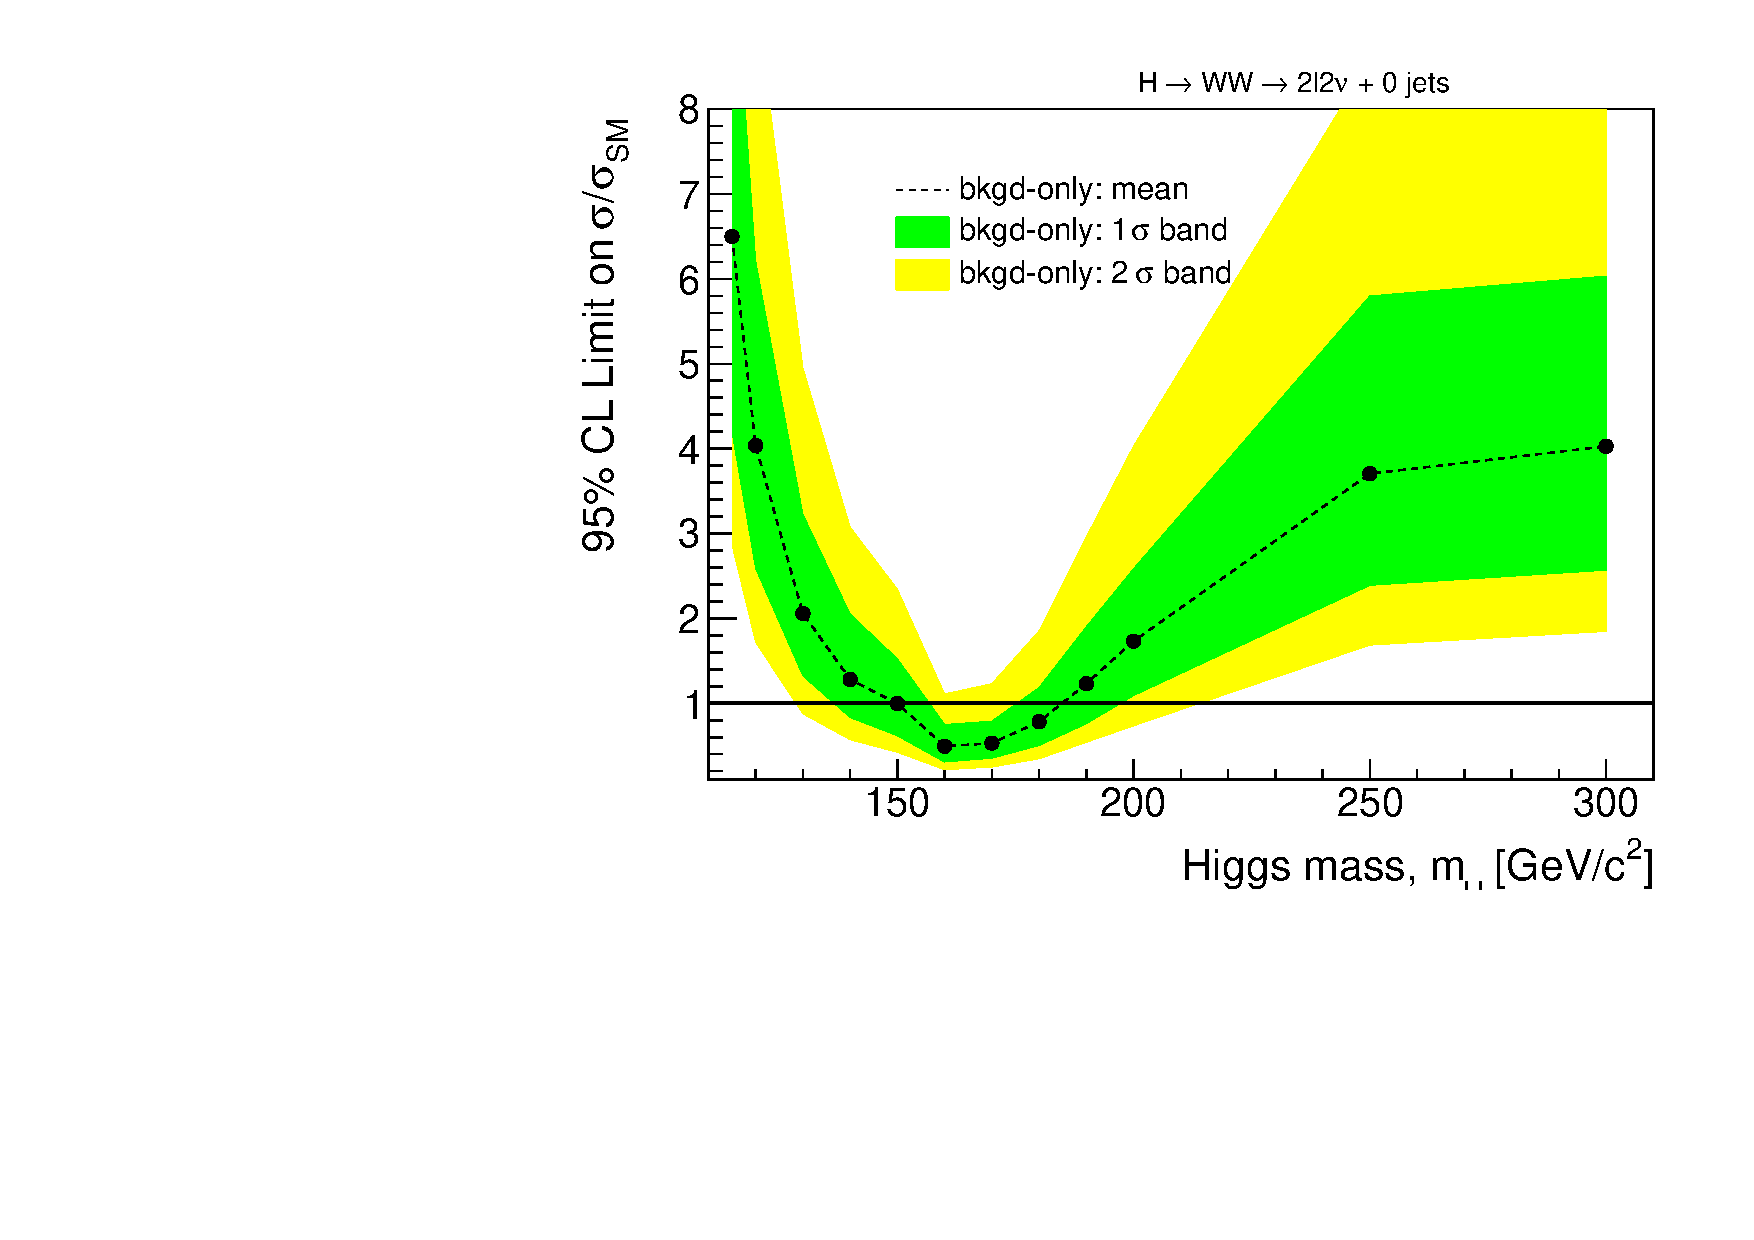
\includegraphics[width=0.49\textwidth]{figures/limits_0j_1000pb_datalike_cut_1.pdf}
   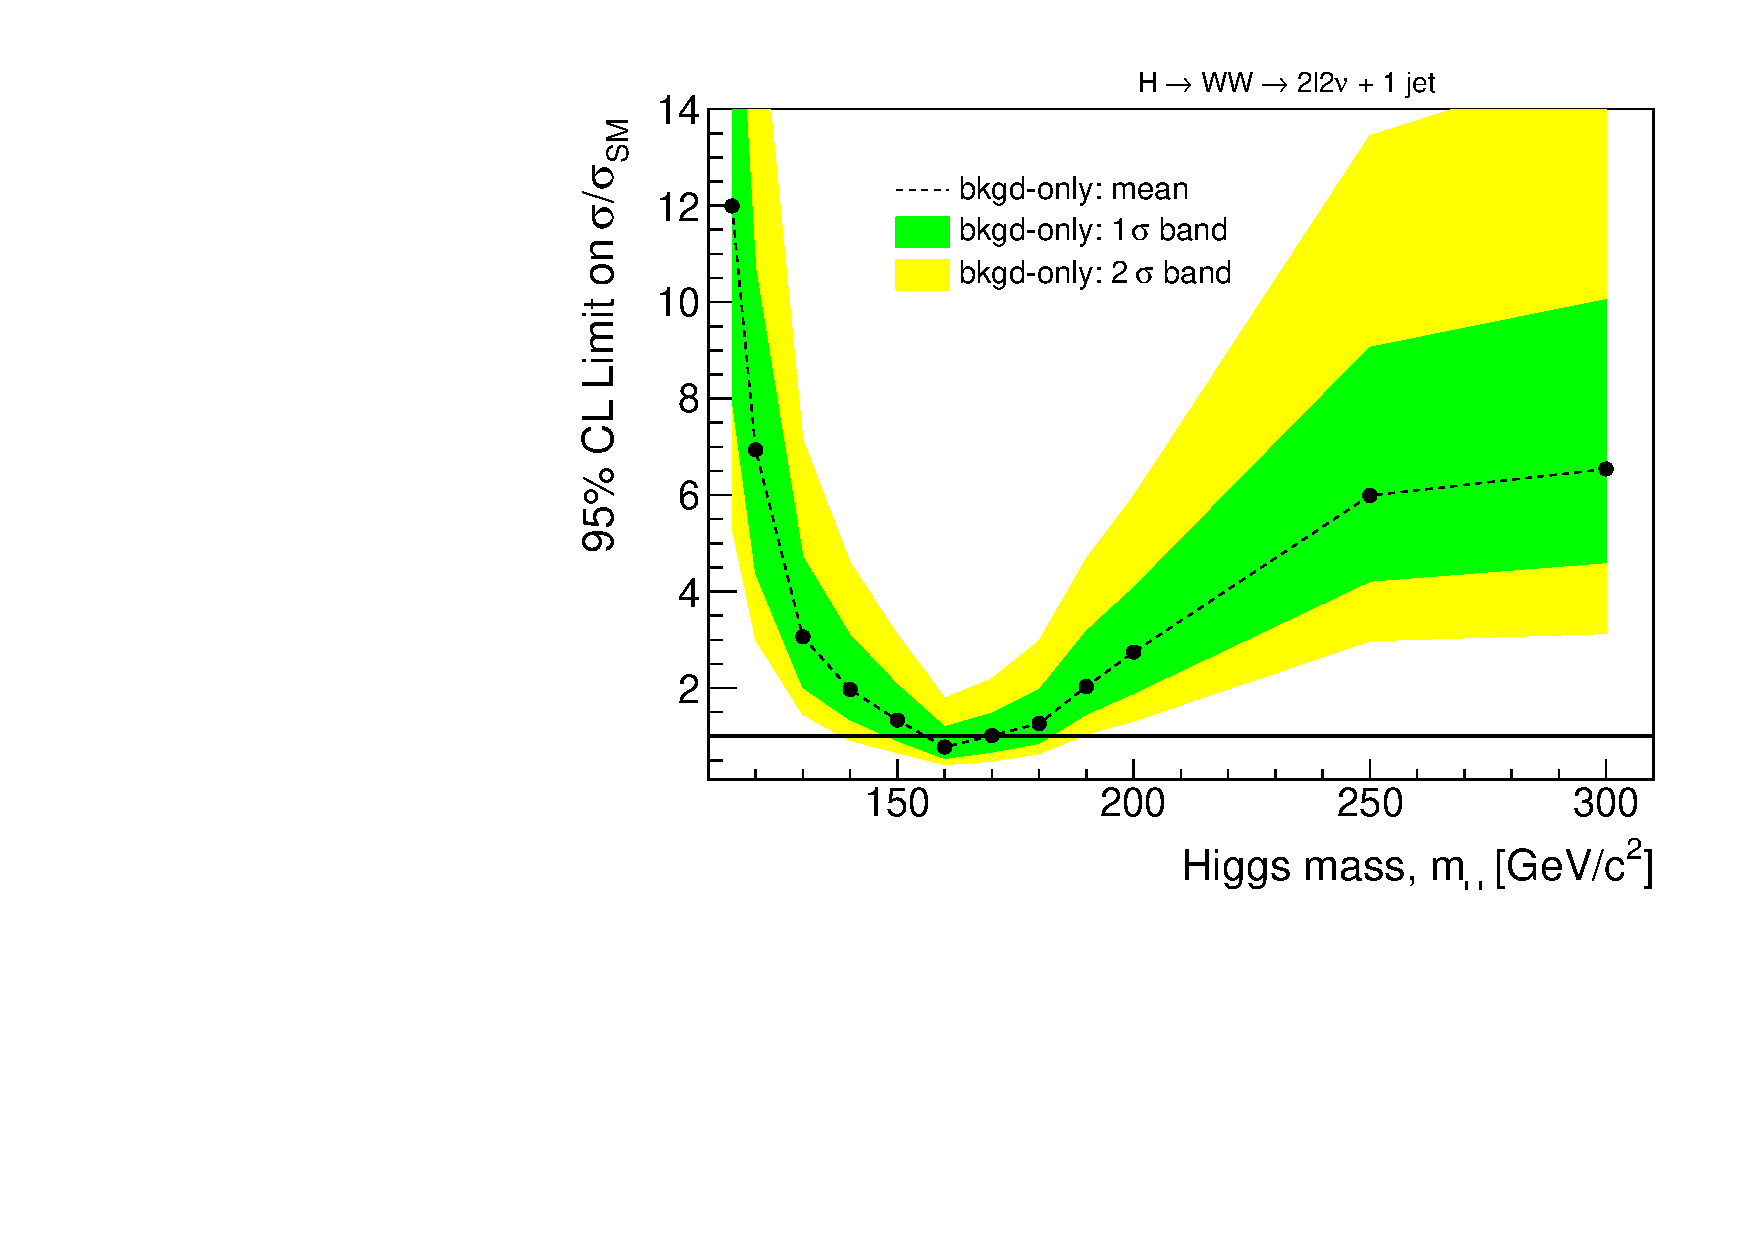
\includegraphics[width=0.49\textwidth]{figures/limits_1j_1000pb_datalike_cut_1.pdf}
   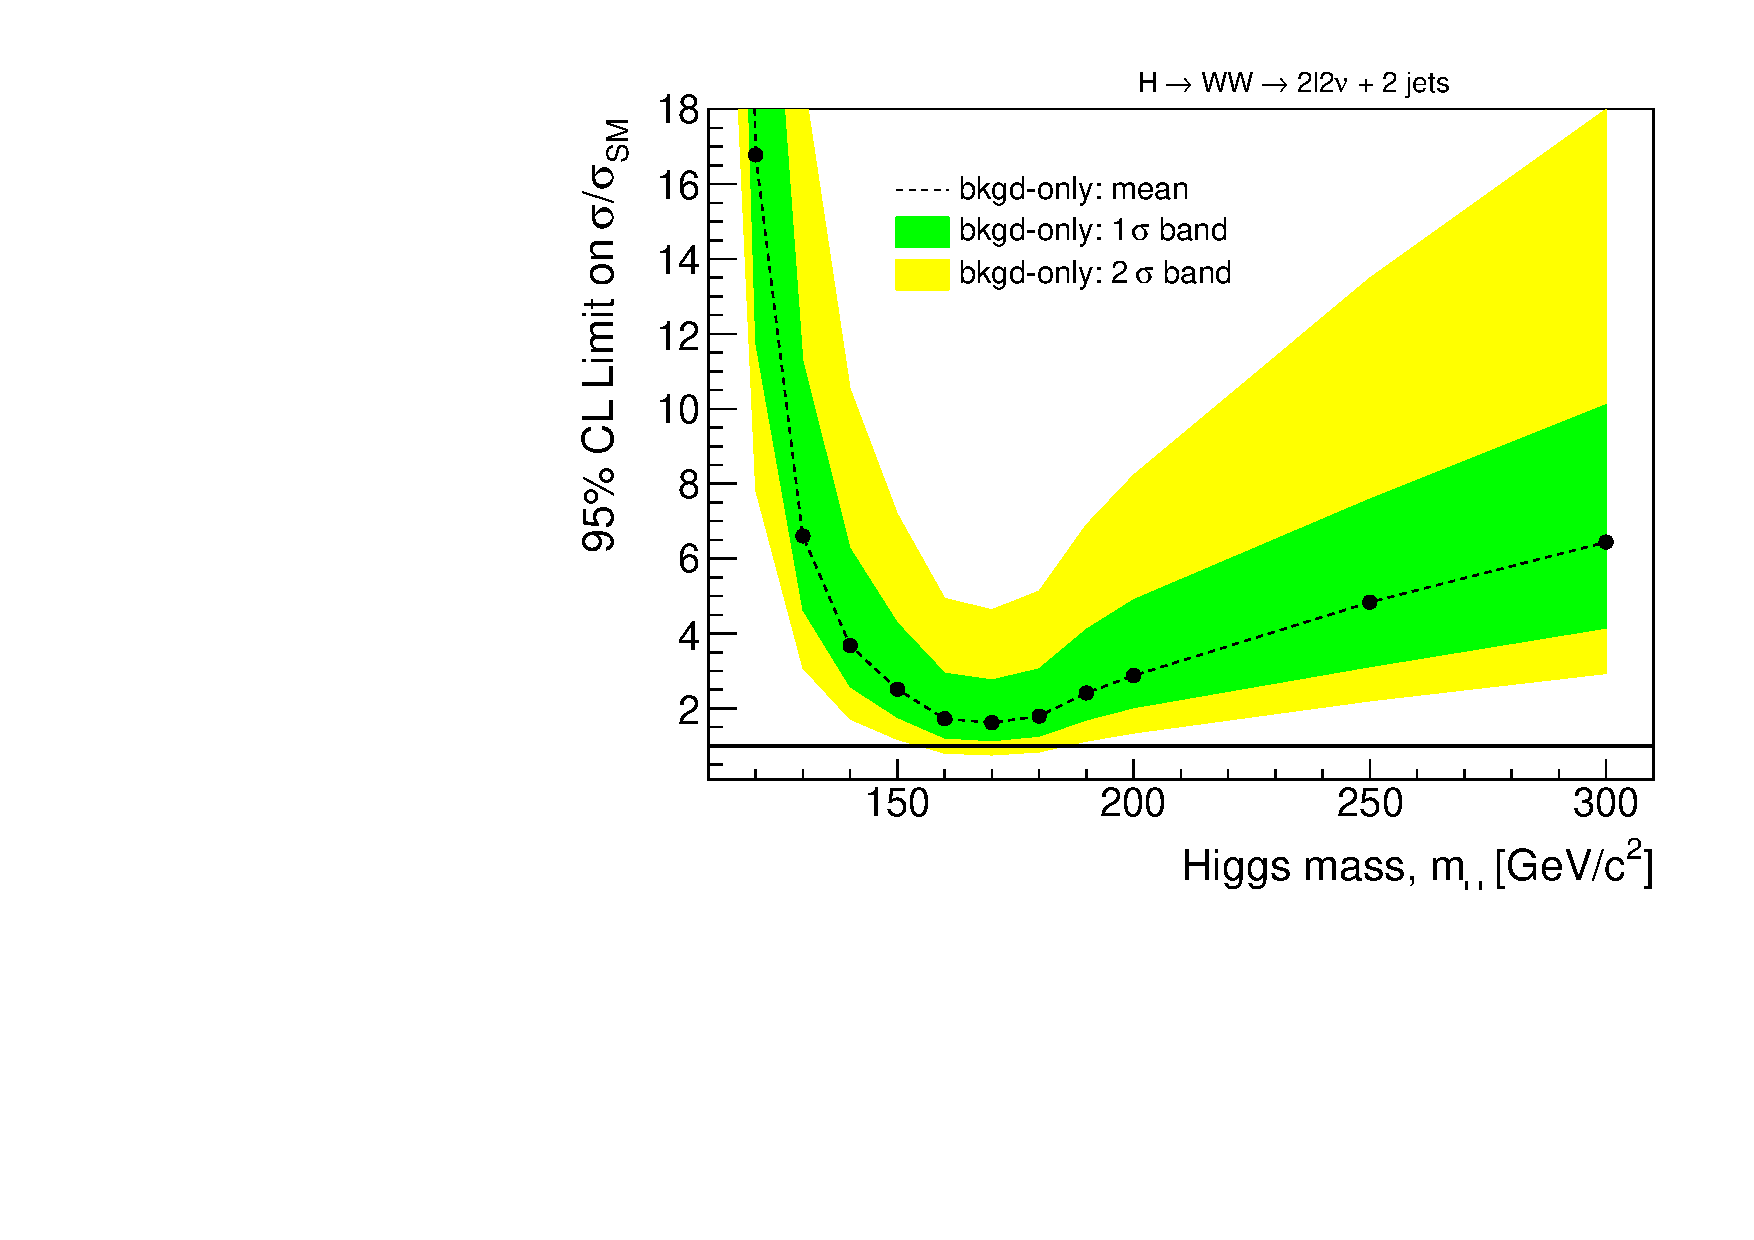
\includegraphics[width=0.49\textwidth]{figures/limits_2j_1000pb_datalike_cut_1.pdf}
   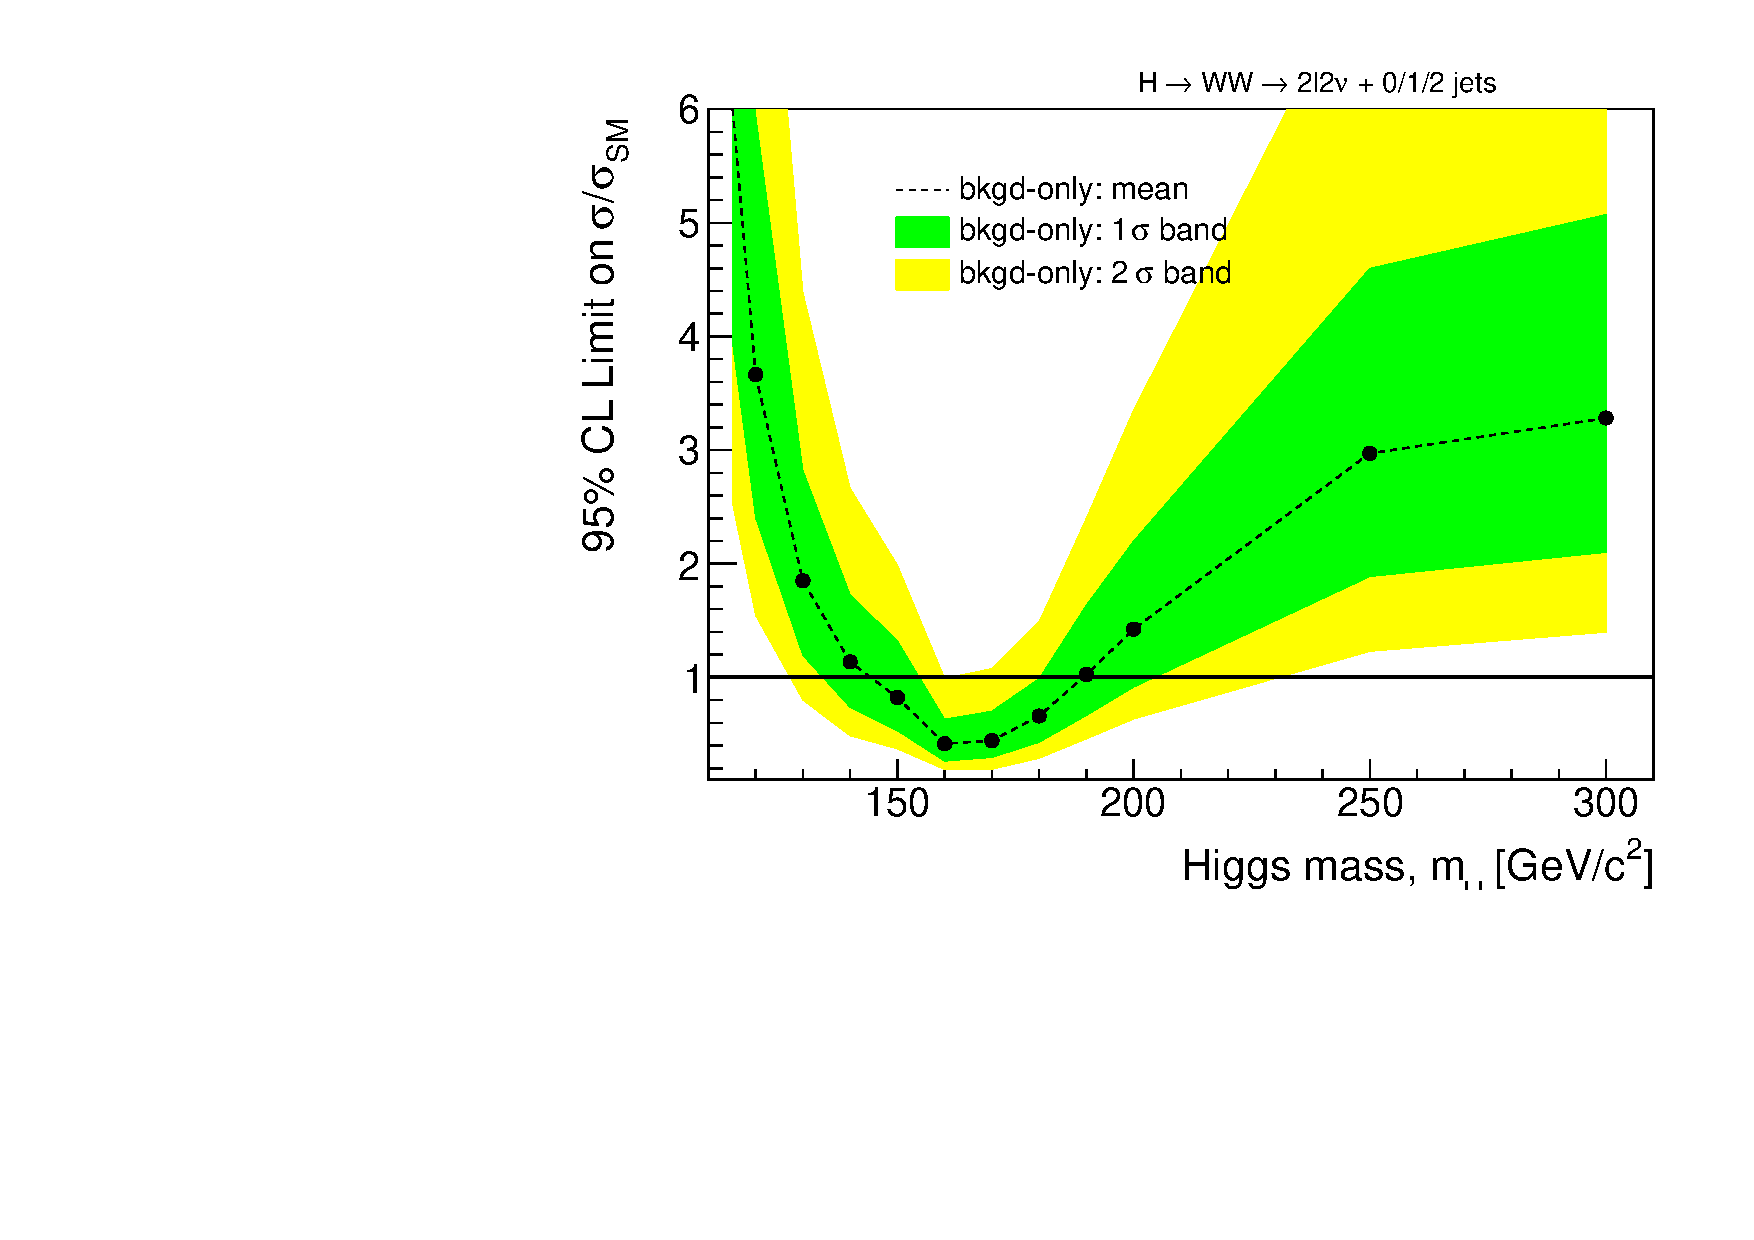
\includegraphics[width=0.49\textwidth]{figures/limits_nj_1000pb_datalike_cut_1.pdf}
   \caption{Cut based analysis expected upper limits at 95\% C.L. for 1\ifb\ of data. Top left plot 
   is the result for the 0-jet bin, top right plot is the result for the 1-jet bin, bottom left plot 
   is the result for the 2-jet bin and, bottom right plot is the combined result. The results 
   are based on the signal and backgrounds corrections from data.}
   \label{fig:cutbase_uls_datalike}
\end{center}
\end{figure}

\begin{figure}[!htbp]
\begin{center}
   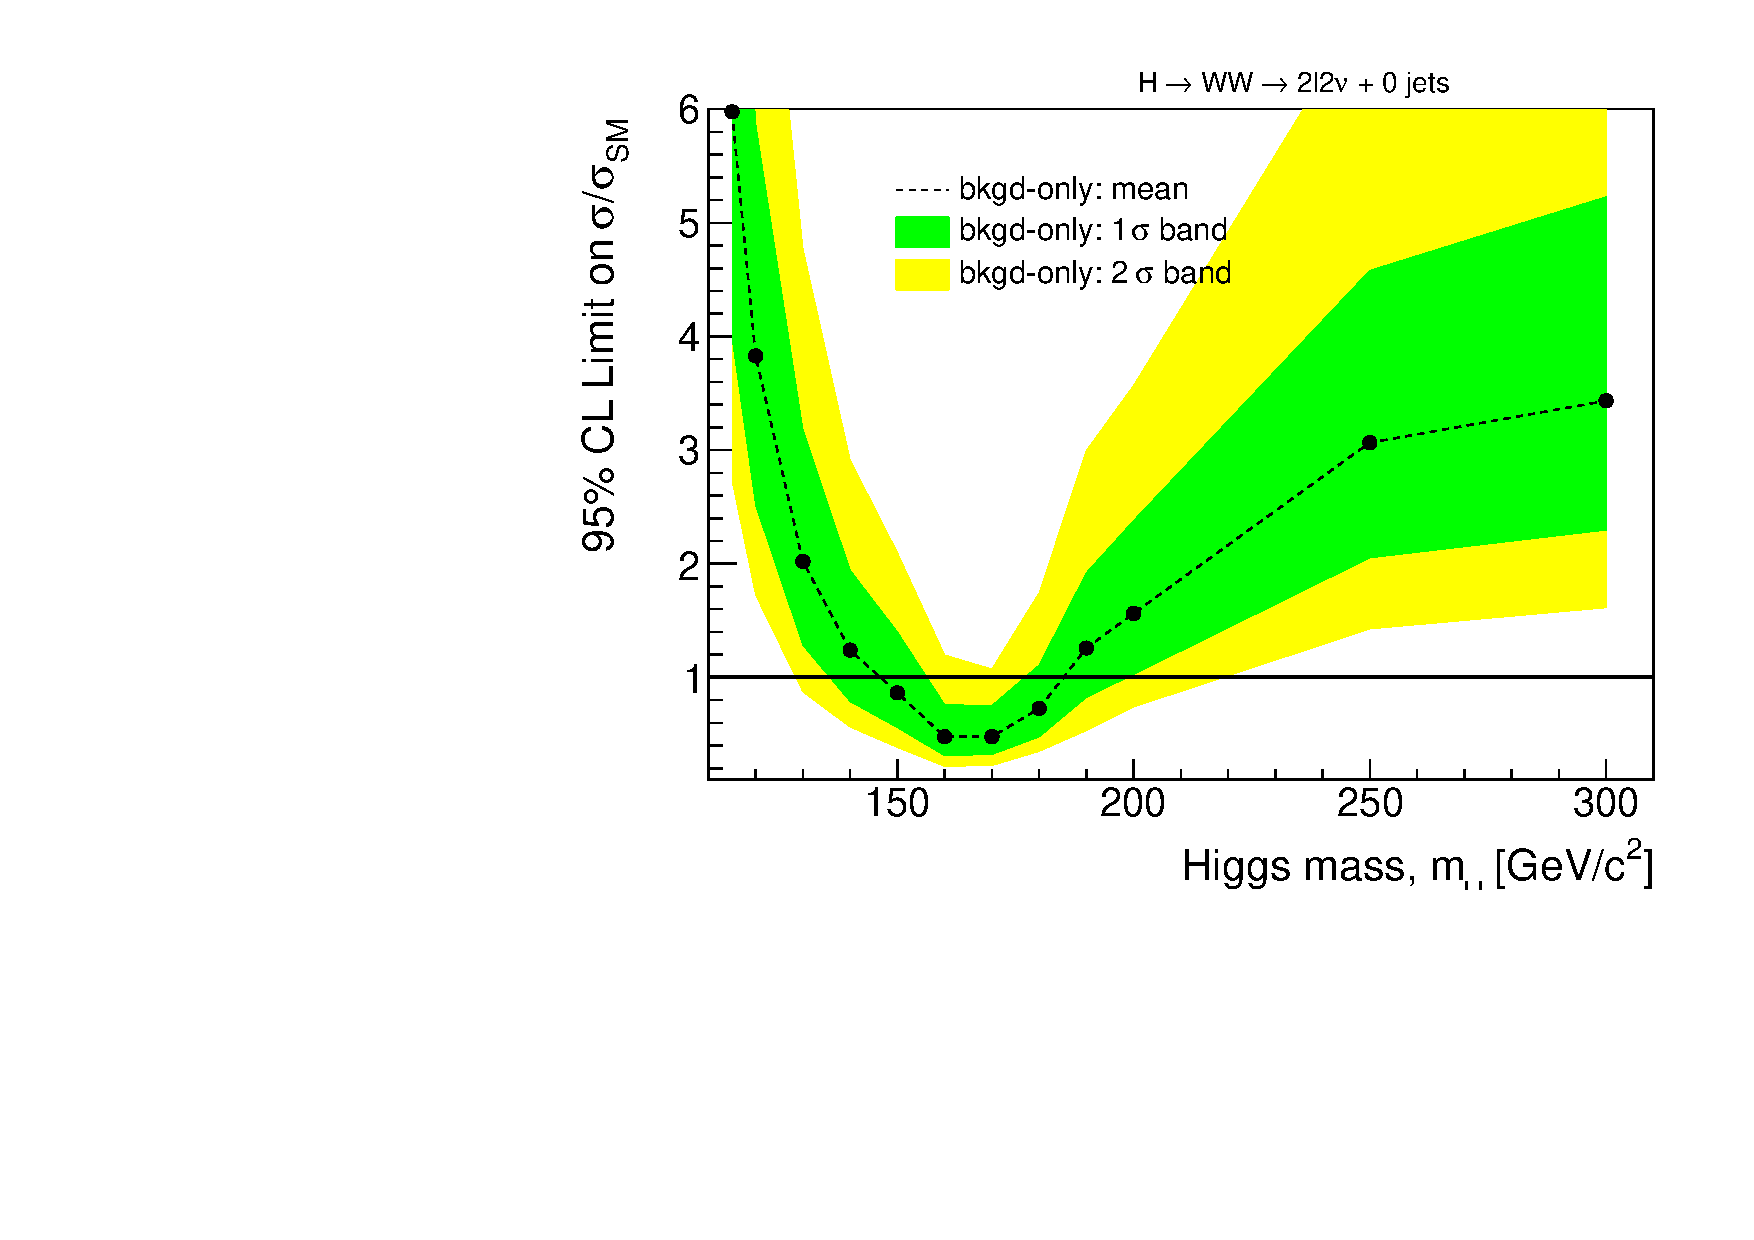
\includegraphics[width=0.49\textwidth]{figures/limits_0j_1000pb_datalike_mva_1.pdf}
   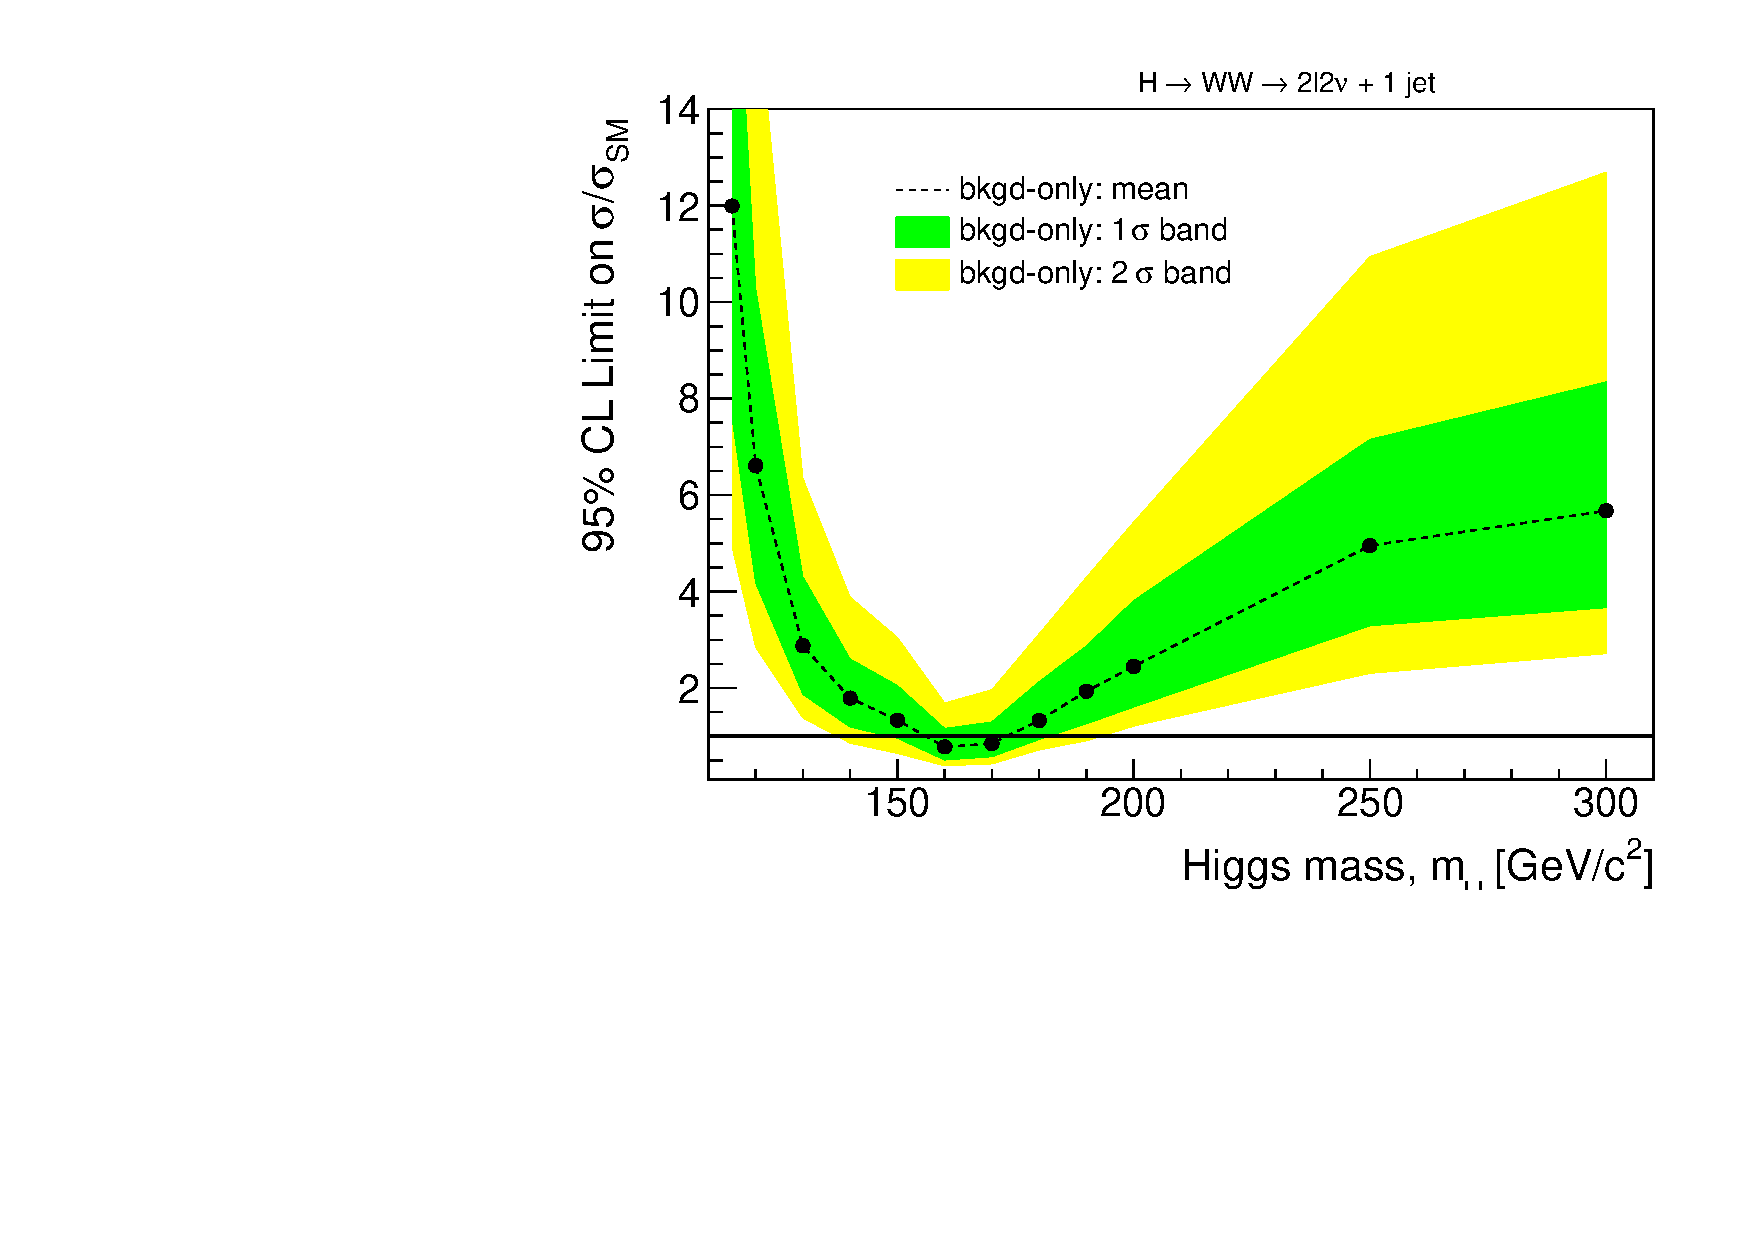
\includegraphics[width=0.49\textwidth]{figures/limits_1j_1000pb_datalike_mva_1.pdf}
   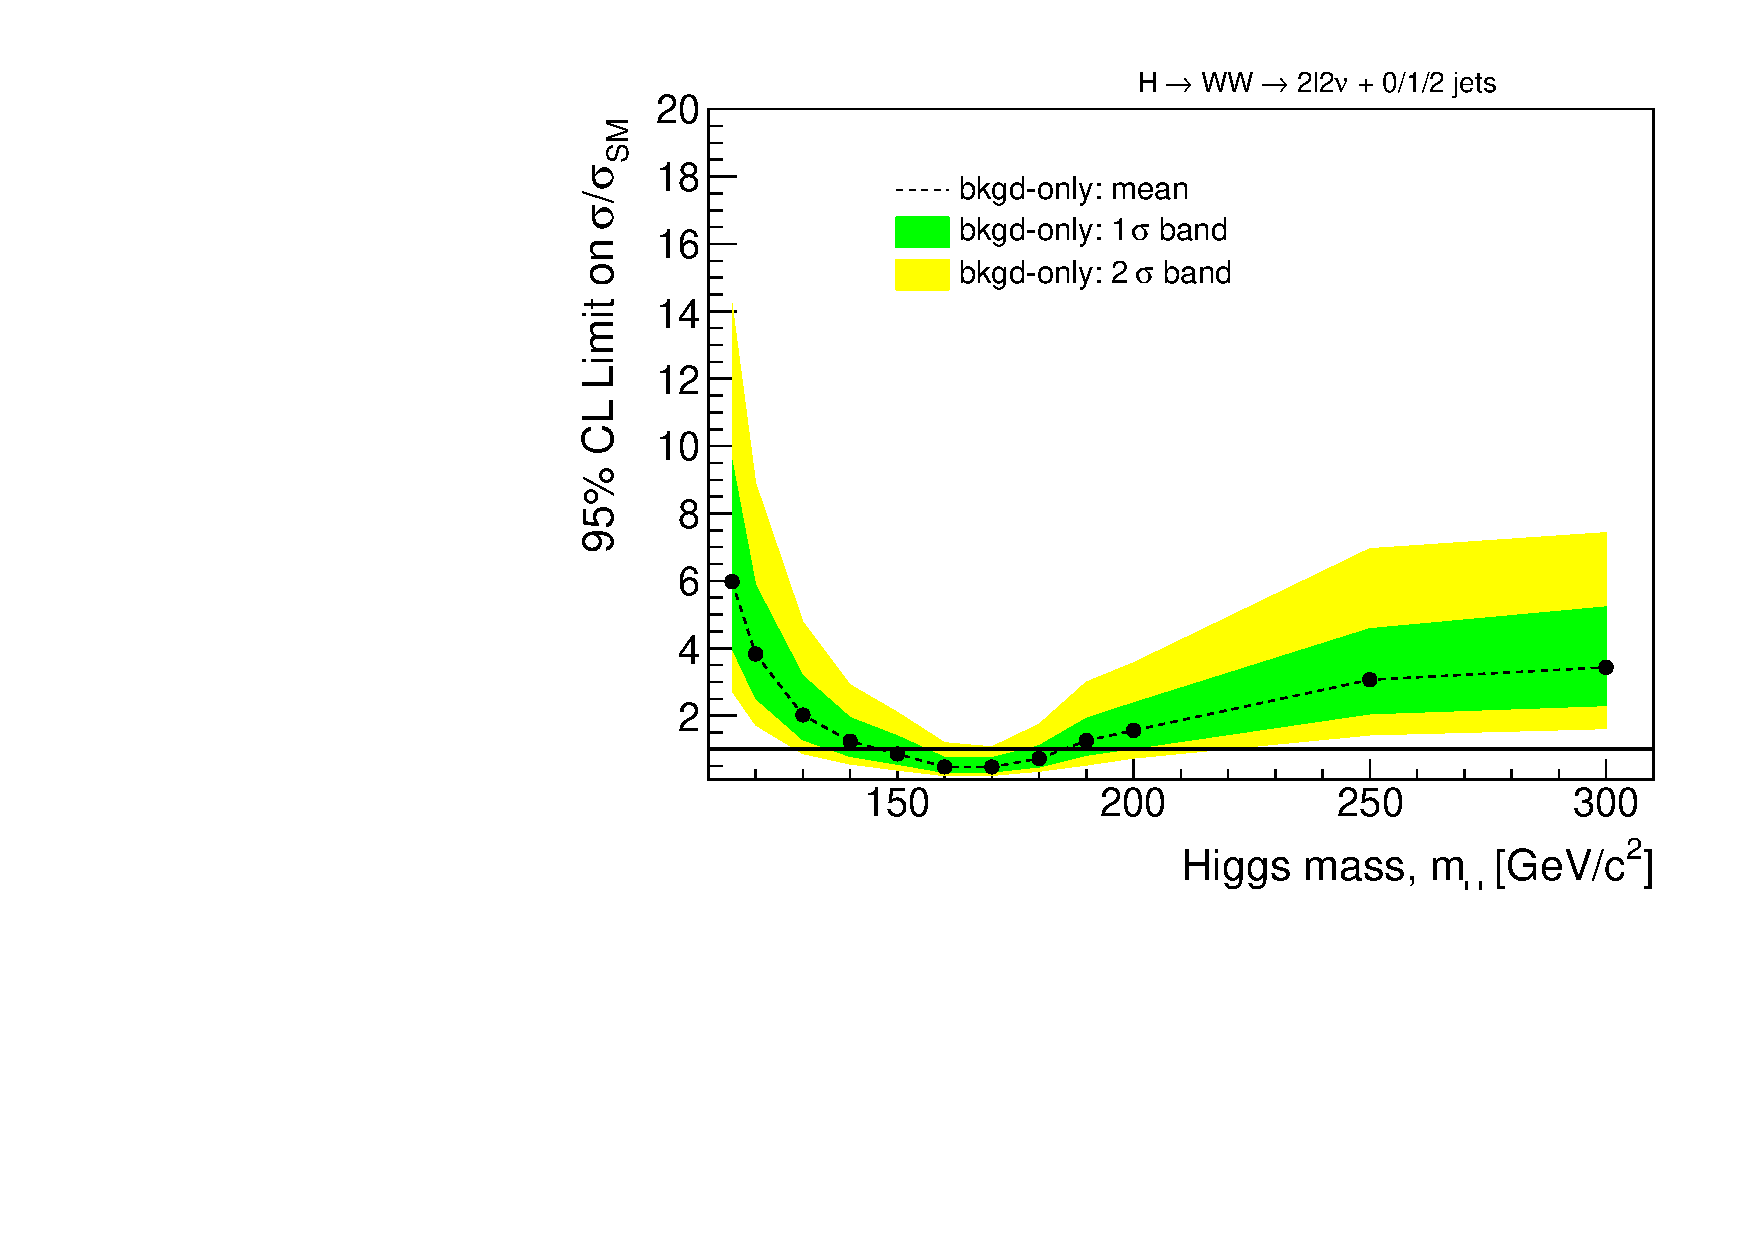
\includegraphics[width=0.49\textwidth]{figures/limits_nj_1000pb_datalike_mva_1.pdf}
   \caption{Multivariate cut-based analysis expected upper limits at 95\% C.L. for 1\ifb\ of data. Top left plot 
   is the result for the 0-jet bin, top right plot is the result for the 1-jet bin, and 
   bottom plot is the combined result including the cut based 2-jet bin analysis. The results 
   are based on the signal and backgrounds corrections from data.}
   \label{fig:mvabase_uls_datalike}
\end{center}
\end{figure}

\begin{figure}[!htbp]
\begin{center}
   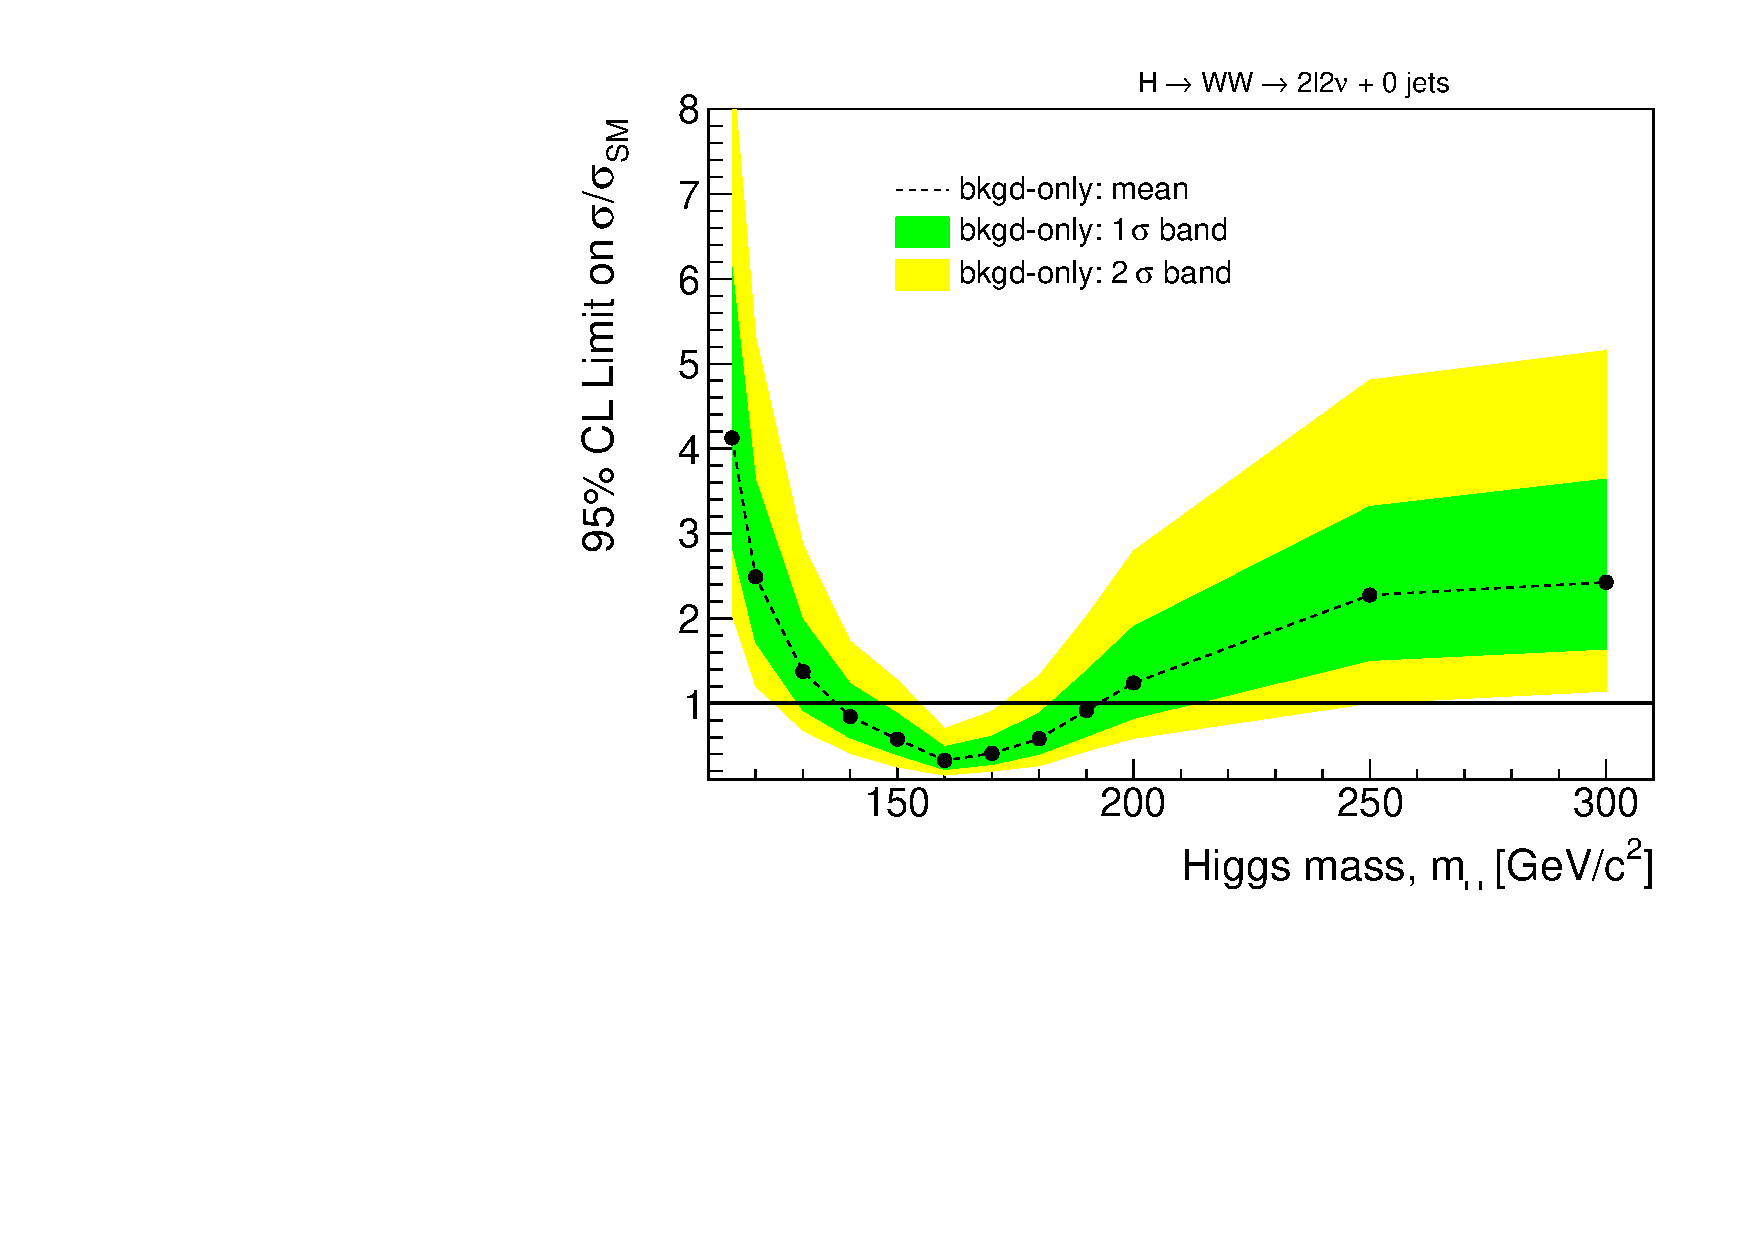
\includegraphics[width=0.49\textwidth]{figures/limits_0j_1000pb_datalike_shape_1.pdf}
   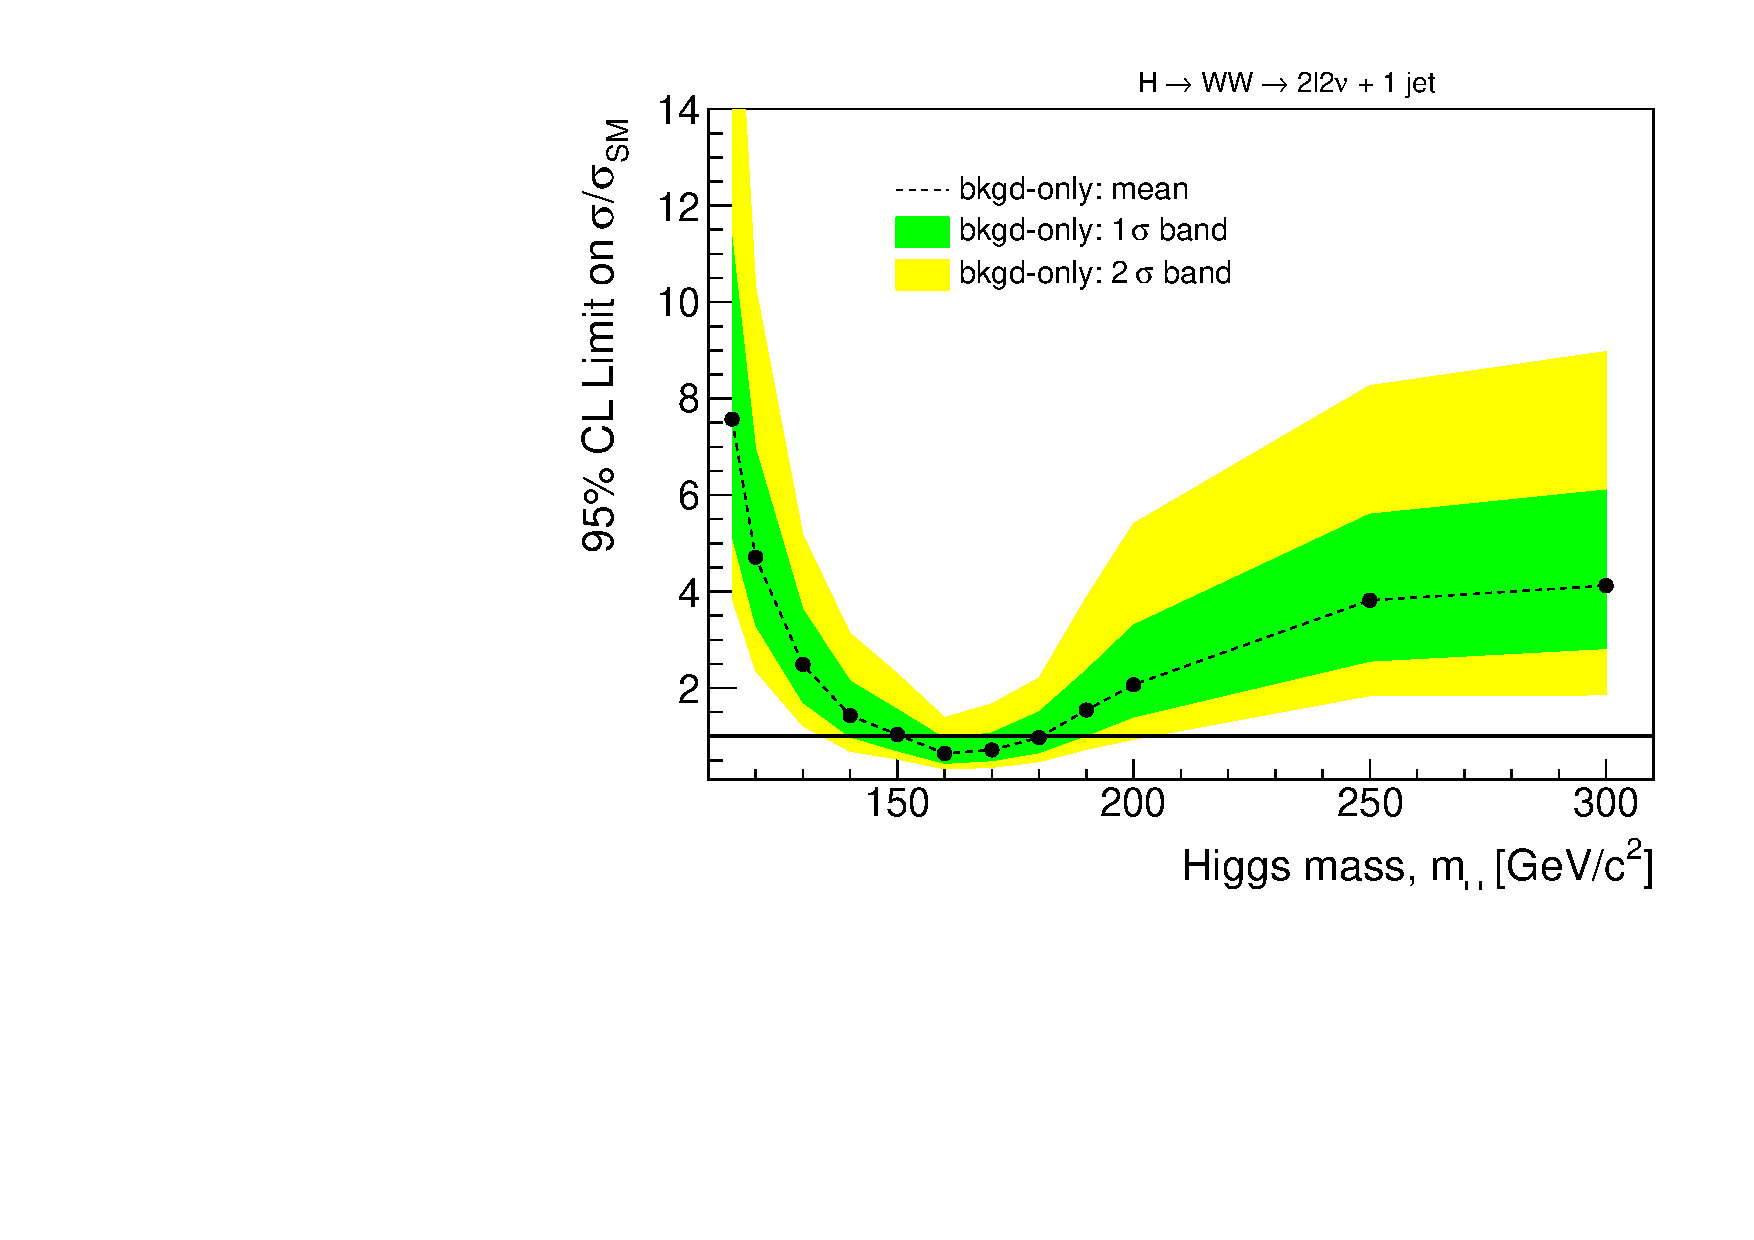
\includegraphics[width=0.49\textwidth]{figures/limits_1j_1000pb_datalike_shape_1.pdf}
   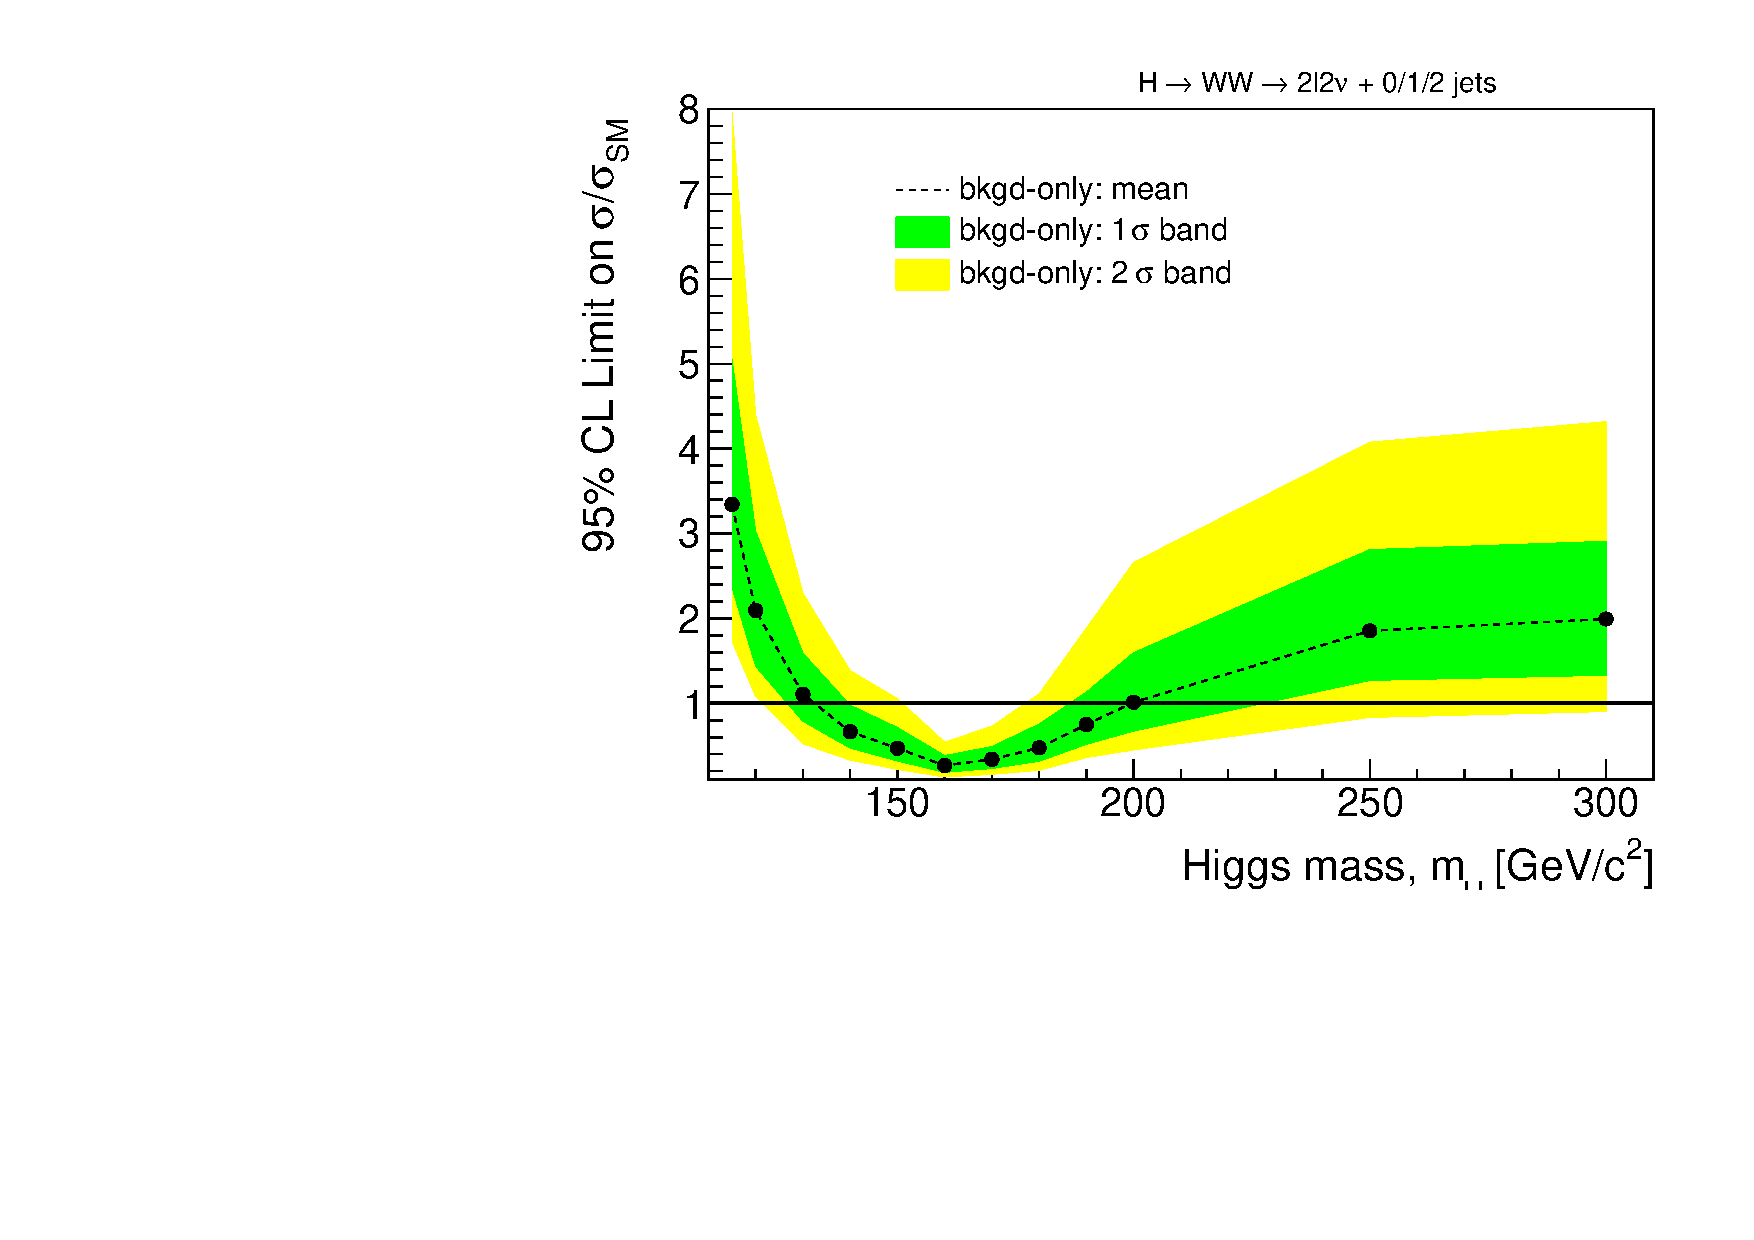
\includegraphics[width=0.49\textwidth]{figures/limits_nj_1000pb_datalike_shape_1.pdf}
   \caption{Multivariate shape analysis expected upper limits at 95\% C.L. for 1\ifb\ of data. Top left plot 
   is the result for the 0-jet bin, top right plot is the result for the 1-jet bin, and 
   bottom plot is the combined results. The results 
   are based on the signal and backgrounds corrections from data.}
   \label{fig:mvashape_uls_datalike}
\end{center}
\end{figure}

